\section{Performance Evaluation} \label{evaluation}
In this article, we have proposed two novel tree-based solutions for static and incremental mining problems, namely Tree-Miner based on SP-Tree and IncTree-Miner based on IncSP-Tree. So, during comparison, we considered those popular and state-of-the-art algorithms which were designed as a new mining technique to solve this problem. We also designed a new support counting strategy which helps detect patterns' infrequency early along with some additional pruning strategies.

To compare Tree-Miner, we have considered three popular state-of-the-art mining algorithms, PrefixSpan\cite{han2001prefixspan}, CM-SPAM and CM-SPADE\cite{fournier2014fast} and to compare IncTree-Miner we considered IncSP\cite{lin2004incremental} and PBIncSpan \cite{chen2007incremental}. We have chosen IncSP and PBIncSpan because they are two of the most prominent mining techniques to solve ISPM problem. As these are based on a single minimum support threshold parameter and has similar key factors, there is a solid ground to compare with. We have introduced a new mining approach, so we considered those which did the same. All the implementations were in Python language and the experiments were conducted on a 64-bit machine having Intel Core i5-8265U CPU @ 3.90GHz $\times$ 8, 32 GB RAM, Windows 10 OS.


\subsection{Dataset Description and Parameters}



We have experimented our proposed solutions over various real-life and synthetic datasets. The performance was consistent and matched our intuition.  To discuss the performance we will use the results of the datasets shown in the Table \ref{table:dataset_information_summary}. We have shown the necessary and important information for each dataset in Table \ref{table:dataset_information_summary}. All the real-life datasets are collected from SPMF: A Java Open Source Data Mining Library\footnote{\url{https://www.philippe-fournier-viger.com/spmf/index.php?link=datasets.php}} and synthetic datasets are generated using \textit{IBM Generator} by applying different parameters. In the real-life datasets, all the events had only one single item, so we randomly merged consecutive events to construct multiple itemed events. In Table \ref{table:dataset_information_summary}, we have also shown the average number of itemsets in each sequence ($C$) and average number of items per itemset ($T$) for each dataset after the described modification.

To evaluate our incremental solution, we had to create an incremental mining scenario. To construct the incremental database and represent the common phenomena, we followed the approach mentioned in the relevant literature \cite{lin2004incremental}. Initially, We had the raw database $D_{raw}$, we divided it into two databases, old database $D$ and incremental database $db$. Final updated database was $D^{\prime}$. We have given description of the used variables in Table \ref{table:variables_description}. To understand how the variables work here, we can construct an example using Table \ref{table:static_database} and \ref{table:incremental_database}. Here Table \ref{table:static_database} will work as $D_{raw}$, first iteration of Table \ref{table:incremental_database} will work as $D$ and second iteration of Table \ref{table:incremental_database} will work as $db$. $D_{Append}$ contains 2 sequences or sids ($sid=1$ and $sid=4$) and $D_{Insert}$ contains 4 sequences ($sid=7,8,9,10$). So here $R_{new}=\frac{4\times100}{10}\%=40\%$, $R_{com}=\frac{2 \times 100}{10}\%=20\%$ and $R_{prev}=\frac{(\frac{5}{8}+\frac{2}{5})\times 100\%}{2}=51.25\%$. Here $\frac{5}{8}$ comes from sequence 1 ($sid=1$) which means in the total length of 8 items 5 items appeared in the first pass and the remaining 3 items in the second pass. Same concept applies for $\frac{2}{5}$ for the sequence 4. For conducting experiments, for each dataset, we chose $R_{new}=10\%, R_{com}=50\%$ and $R_{prev}=80\%$ similar to \cite{lin2004incremental}. 



We have defined density ratio of a dataset as $d^{*} = \frac{\text{avg. sequence length} \times 100}{\text{(\#)unique items}}$ which is the combination of average sequence length and number of unique items. To evaluate our proposals we have used datasets of both types, highly densed (with high ratio of $d^{*}$) and comparatively much lesser densed. 



\begin{table*}[!htb]
%% increase table row spacing, adjust to taste
%\renewcommand{\arraystretch}{1.3}
% if using array.sty, it might be a good idea to tweak the value of
% \extrarowheight as needed to properly center the text within the cells
\centering
%% Some packages, such as MDW tools, offer better commands for making tables
%% than the plain LaTeX2e tabular which is used here.
\begin{tabular}{|c|c|c|c|c|c|c|c|}
\hline
Name & Description & Sequence & Unique & Avg. sequ- & \textit{C} & \textit{T} & $d^{*}$\\
& & Count & Items & ence Length & & &\\ 
\hline
Bible & Conversion of Bible & 36,369 & 13,905 & 21.64  &  10.97 & 15.49 & 0.16 \\
\hline
MSNBC & Click Stream & 31790 & 17 & 13.23 & 7.83 & 10.81 & 77.82\\ 
\hline
BMSWebView1 & Click Stream & 59601 & 497 & 2.43 & 2.19 & 6.2 & 0.49\\ 
\hline
Sign & Sign Language & 730 & 267  & 51.997 & 25.99 & 28.49 & 19.47\\ 
\hline
Kosarak & Click Stream & 990000 & 41270 & 8.1 & 3.7 & 6.23 & 0.02\\ 
\hline
L20k-C10-T5-N1K & Synthetic Dataset & 20000 & 1000 & 44.21 &  10 & 5 & 4.42\\ 
\hline
L50k-C10-T2.5-N10K  & Synthetic Dataset &  50000 & 10000  & 21.79 & 10 & 2.5 & 0.22\\ 
\hline
\end{tabular}
\caption{Dataset Summarized Information}
\label{table:dataset_information_summary}
\end{table*}


\begin{table*}[!t]
\centering
%% increase table row spacing, adjust to taste
%\renewcommand{\arraystretch}{1.3}
% if using array.sty, it might be a good idea to tweak the value of
% \extrarowheight as needed to properly center the text within the cells
%\centering
%% Some packages, such as MDW tools, offer better commands for making tables
%% than the plain LaTeX2e tabular which is used here.
\begin{tabular}{|l|l|}
\hline
Variable & Description\\ \hline 
$D$ & Old database \\ \hline
$db$ & Incremental database, $db=D_{Insert} \cup D_{Append}$. \\ \hline
$D^{\prime}$ & Updated database, $D^{\prime}=D \cup db$.\\ \hline
$R_{new}$ & \textit{New sequence Ratio: }Percentage of sequences completely removed from $D_{raw}$ to put in $D_{Insert}$.\\
&   $|D_{Insert}|=R_{new} \times |D_{raw}|$\\
\hline
$R_{com}$ & \textit{Common Sequence Ratio: }Percentage of common sids picked from $D_{raw}$ to put into $D$ and $D_{Append}$.  \\
& $|D_{Append}| = R_{com} \times |D_{raw}|$.\\ 
\hline
$R_{prev}$ & \textit{Previous Appearing Ratio: }Avg. splitting ratio for the common sequences lying in  $D$ and $D_{Append}$. \\
& If $R_{prev}=80\%$, then for each common sequence (in avg.) $80\%$ items will be in $D$ and $20\%$ will be \\
& in $D_{Append}$. \\
\hline
$L$ & Total Number of sequences\\ \hline
$C$ & Avg. number of itemsets per sequence \\ \hline 
$T$ & Avg. Number of items in each itemset \\ \hline 
$N$ & Number of distinct Items \\ \hline
\end{tabular}
\caption{Variables' Description}
\label{table:variables_description}
\end{table*}




\subsection{Tree-Miner}
In this section, we will evaluate Tree-Miner based on various metrics and analyze the results. 

\subsubsection{Runtime, Memory Usage and Scalability}
In Fig. \ref{graph:runtime_scalability_comparison_tree_miner} (a)-(g) we present the runtime performance of Tree-Miner. From the corresponding figures, it is obvious that our proposed Tree-Miner based on SP-Tree performs comparatively better than other static mining algorithms. SP-Tree is a compact representation of the database which provides huge structural control over it. Through the next links, we perform efficient traversals in the database which ultimately helps to generate the patterns faster. We also use a set of pruning techniques that significantly reduce the search space. We adopted all the previous pruning techniques and also incorporated some newer ones which makes it a very efficient mining algorithm. In the figures, in lower thresholds, our performance improvement is quite visible because we need to encounter a huge number of patterns and Tree-Miner efficiently discovers them whereas in upper thresholds the performance is quite close because the number of patterns is very small. The performance gets improved in dense datasets through node overlapping characteristics and in sparse datasets through faster database reduction and projection though next links. Our SP-Tree structure is enough to calculate the complete support of the patterns having no necessity to maintain additional structure for each pattern which is also an important factor to improve performance. In Fig. \ref{graph:runtime_scalability_comparison_tree_miner} (a)-(g) we have shown the results for Sign, Bible, BmsWebView1, MSNBC, Kosarak, L20k-C10-T5-N1K and L50k-C10-T2.5-N10K datasets respectively. 


\begin{figure*}[!tb]
         \centering
        \begin{subfigure}{.3\linewidth}
         \centering
        \begin{adjustbox}{max width=\textwidth}
         %sign dataset 
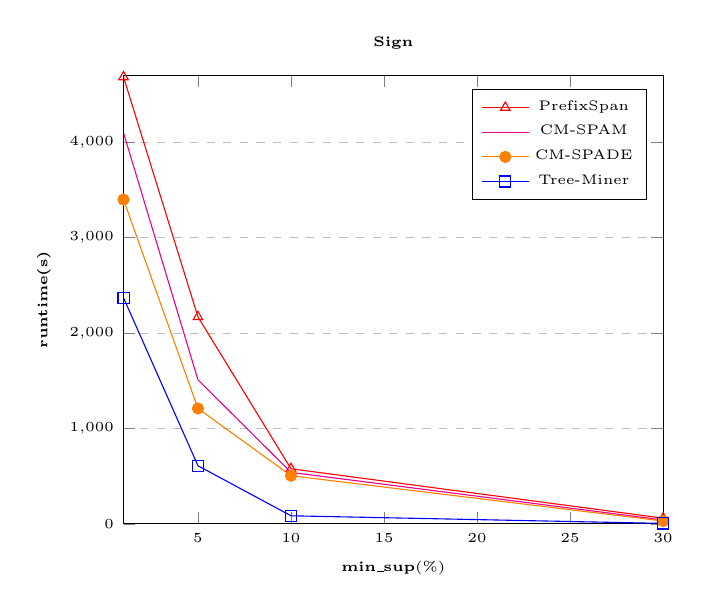
\begin{tikzpicture}
\begin{axis}[
    title={\textbf{Sign}},
    xlabel={$\textbf{min\_sup}$(\%)},
    ylabel={\textbf{runtime(s)}},
    xmin=1, xmax=30,
    ymin=0, ymax=4700,
    %xtick={41, 43, 45, 47, 49, 51, 53, 55},
    %ytick={20, 30, 40, 50, 60, 70, 80, 90, 100, 110, 120, 130, 140},
    legend pos=north east,
    ymajorgrids=true,
    grid style=dashed,
    legend style={font=\tiny},
    title style={font=\tiny},
    label style={font=\tiny},
    every tick label/.append style={font=\tiny}
]
%(41, 12)
%(47, 9)
%(55, 7)
%tree-miner
  \addplot[
    color=red,
    mark=triangle,
    ]
    coordinates {
        (30, 60) 
        (10, 578)
        (5, 2170)
        (1, 4685)
    };
    \addlegendentry{PrefixSpan}
    
    \addplot[
    color=magenta,
    ]
    coordinates {
        (30, 41) 
        (10, 540)
        (5, 1510)
        (1, 4100)
    };
    \addlegendentry{CM-SPAM}
    
    \addplot[
    color=orange,
    mark=*,
    ]
    coordinates {
        (30, 30) 
        (10, 505)
        (5, 1210)
        (1, 3400)
    };
    \addlegendentry{CM-SPADE}
    
    \addplot[
    color=blue,
    mark=square,
    ]
    coordinates {
        (30, 5) 
        (10, 85)
        (5, 610)
        (1, 2370)
    };
    \addlegendentry{Tree-Miner}
\end{axis}
\end{tikzpicture}
        \end{adjustbox}
        \caption{}
        \end{subfigure}
        \begin{subfigure}{.3\linewidth}
          \centering
        \begin{adjustbox}{max width=\textwidth}
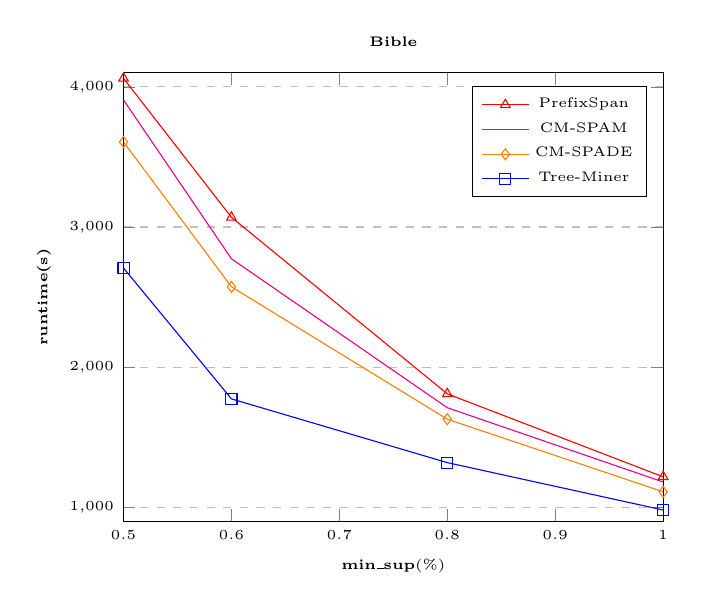
\begin{tikzpicture}
\begin{axis}[
    title={\textbf{Bible}},
   xlabel={$\textbf{min\_sup}$(\%)},
    ylabel={\textbf{runtime(s)}},
    xmin=0.5, xmax=1,
    ymin=900, ymax=4100,
    %xtick={500, 600, 700, 800, 900, 1000},
    %ytick={250, 350, 450, 550, 650, 750, 850, 950, 1050, 1150, 1250, 1350, 1450},
    legend pos=north east,
    ymajorgrids=true,
    grid style=dashed,
    legend style={font=\tiny},
    title style={font=\tiny},
    label style={font=\tiny},
    every tick label/.append style={font=\tiny}
]

%prefixspan
\addplot[
    color=red,
    mark=triangle,
    ]
    coordinates {
        (0.5, 4061) 
        (0.6, 3069)
        (0.8, 1809)
        (1, 1217)
    };
    \addlegendentry{PrefixSpan}
    
  \addplot[
    color=magenta
    ]
    coordinates {
        (0.5, 3907) 
        (0.6, 2773)
        (0.8, 1710)
        (1,   1180)
    };
    \addlegendentry{CM-SPAM}
    
    \addplot[
    color=orange,
    mark=diamond,
    ]
    coordinates {
        (0.5, 3607) 
        (0.6, 2573)
        (0.8, 1628)
        (1,   1110)
    };
    \addlegendentry{CM-SPADE}
    
    %tree-miner
    \addplot[
        color=blue,
        mark=square,
        ]
        coordinates {
            (0.5, 2707) 
            (0.6, 1773)
            (0.8, 1318)
            (1,   980)
        };
        \addlegendentry{Tree-Miner}
\end{axis}
\end{tikzpicture}
        \end{adjustbox}
        \caption{}
        \end{subfigure}
        \begin{subfigure}{.3\linewidth}
          \centering
        \begin{adjustbox}{max width=\textwidth}
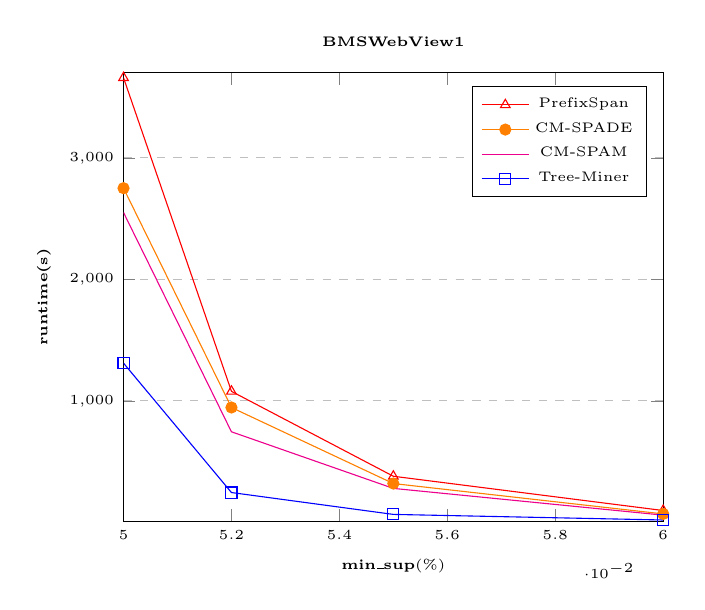
\begin{tikzpicture}
\begin{axis}[
    title={\textbf{BMSWebView1}},
    xlabel={$\textbf{min\_sup}$(\%)},
    ylabel={\textbf{runtime(s)}},
    xmin=0.05, xmax=0.06,
    ymin=10, ymax=3700,
    %xtick={38, 40, 42, 44, 46, 48},
    %ytick={10, 20, 30, 40, 50},
    legend pos=north east,
    ymajorgrids=true,
    grid style=dashed,
    legend style={font=\tiny},
    title style={font=\tiny},
    label style={font=\tiny},
    every tick label/.append style={font=\tiny}
]

\addplot[
    color=red,
    mark=triangle,
    ]
    coordinates {
      (0.06,  98) 
      (0.055, 380)
      (0.052, 1079)
      (0.05,  3660)
    };
    \addlegendentry{PrefixSpan}
    
    \addplot[
    color=orange,
    mark=*
    ]
    coordinates {
        (0.06,  70) 
        (0.055, 320)
        (0.052, 946)
        (0.05,  2751)
    };
    \addlegendentry{CM-SPADE}

\addplot[
    color=magenta
    ]
    coordinates {
        (0.06,  60) 
        (0.055, 280)
        (0.052, 746)
        (0.05,  2551)
    };
    \addlegendentry{CM-SPAM}
    
   
    \addplot[
    color=blue,
    mark=square,
    ]
    coordinates {
        (0.06,  20) 
        (0.055, 66)
        (0.052, 246)
        (0.05,  1311)
    };
    \addlegendentry{Tree-Miner}
\end{axis}
\end{tikzpicture}
        \end{adjustbox}
        \caption{}
        \end{subfigure}
        \begin{subfigure}{.3\linewidth}
          \centering
        \begin{adjustbox}{max width=\textwidth}
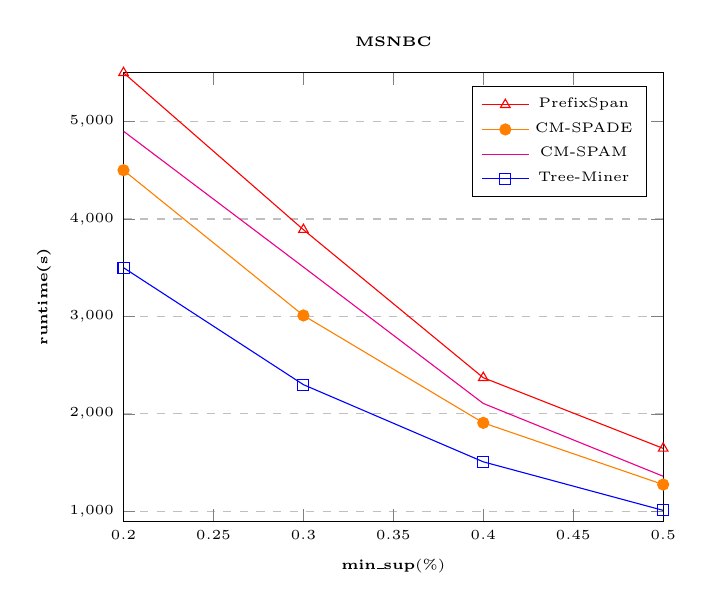
\begin{tikzpicture}
\begin{axis}[
    title={\textbf{MSNBC}},
    xlabel={$\textbf{min\_sup}$(\%)},
    ylabel={\textbf{runtime(s)}},
    xmin=0.2, xmax=0.5,
    ymin=900, ymax=5500,
    %xtick={38, 40, 42, 44, 46, 48},
    %ytick={10, 20, 30, 40, 50},
    legend pos=north east,
    ymajorgrids=true,
    grid style=dashed,
    legend style={font=\tiny},
    title style={font=\tiny},
    label style={font=\tiny},
    every tick label/.append style={font=\tiny}
]

\addplot[
    color=red,
    mark=triangle,
    ]
    coordinates {
        (0.5, 1646) 
        (0.4, 2371)
        (0.3, 3890)
        (0.2, 5500)
    };
    \addlegendentry{PrefixSpan}
    
    \addplot[
    color=orange,
    mark=*
    ]
    coordinates {
        (0.5,  1275) 
        (0.4, 1908)
        (0.3, 3010)
        (0.2, 4500)
    };
    \addlegendentry{CM-SPADE}

\addplot[
    color=magenta
    ]
    coordinates {
        (0.5,  1360) 
        (0.4, 2107)
        (0.3, 3507)
        (0.2, 4900)
    };
    \addlegendentry{CM-SPAM}
    
    
    \addplot[
    color=blue,
    mark=square,
    ]
    coordinates {
        (0.5,  1010) 
        (0.4, 1508)
        (0.3, 2300)
        (0.2,  3500)
    };
    \addlegendentry{Tree-Miner}
\end{axis}
\end{tikzpicture}
        \end{adjustbox}
        \caption{}
        \end{subfigure}
        \begin{subfigure}{.3\linewidth}
          \centering
        \begin{adjustbox}{max width=\textwidth}
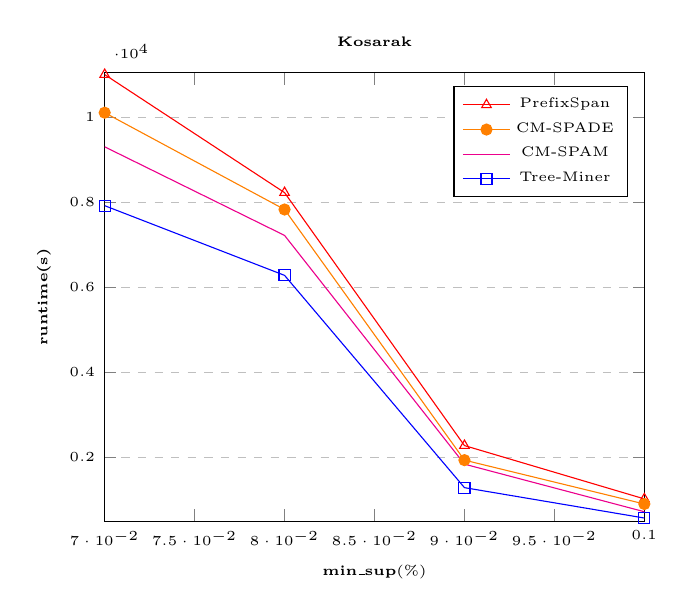
\begin{tikzpicture}
\begin{axis}[
    title={\textbf{Kosarak}},
    xlabel={$\textbf{min\_sup}$(\%)},
    ylabel={\textbf{runtime(s)}},
    xmin=0.07, xmax=0.1,
    ymin=500, ymax=11050,
    %xtick={38, 40, 42, 44, 46, 48},
    %ytick={10, 20, 30, 40, 50},
    legend pos=north east,
    ymajorgrids=true,
    grid style=dashed,
   legend style={font=\tiny},
    title style={font=\tiny},
    label style={font=\tiny},
    every tick label/.append style={font=\tiny}
]

\addplot[
    color=red,
    mark=triangle,
    ]
    coordinates {
        (0.1,   1025)
        (0.09,  2280)
        (0.08,  8232)
        (0.07,  11010)
    };
    \addlegendentry{PrefixSpan}
    
    \addplot[
    color=orange,
    mark=*
    ]
    coordinates {
        (0.1,905)
        (0.09,1937)
        (0.08,7835)
        (0.07,10113)
    };
    \addlegendentry{CM-SPADE}

  \addplot[
    color=magenta
    ]
    coordinates {
        (0.1,723)
        (0.09,1843)
        (0.08,7225)
        (0.07,9310)
    };
    \addlegendentry{CM-SPAM}
    
   
    \addplot[
    color=blue,
    mark=square,
    ]
    coordinates {
        (0.1,575)
        (0.09,1290)
        (0.08,6285)
        (0.07,7925)
    };
    \addlegendentry{Tree-Miner}
\end{axis}
\end{tikzpicture}
        \end{adjustbox}
         \caption{}
        \end{subfigure}
        \begin{subfigure}{.3\linewidth}
          \centering
        \begin{adjustbox}{max width=\textwidth}
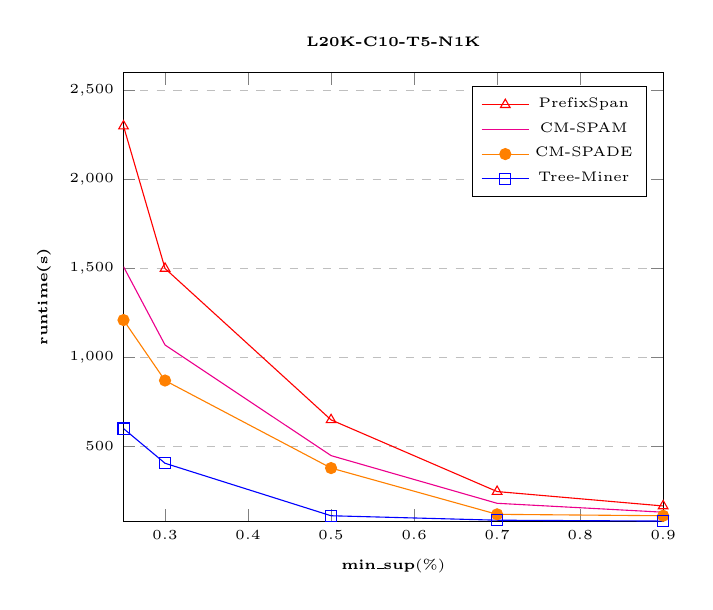
\begin{tikzpicture}
\begin{axis}[
    title={\textbf{L20K-C10-T5-N1K}},
    xlabel={$\textbf{min\_sup}$(\%)},
    ylabel={\textbf{runtime(s)}},
    xmin=0.25, xmax=0.9,
    ymin=80, ymax=2600,
    %xtick={38, 40, 42, 44, 46, 48},
    %ytick={10, 20, 30, 40, 50},
    legend pos=north east,
    ymajorgrids=true,
    grid style=dashed,
    legend style={font=\tiny},
    title style={font=\tiny},
    label style={font=\tiny},
    every tick label/.append style={font=\tiny}
]

\addplot[
    color=red,
    mark=triangle,
    ]
    coordinates {
        (0.9,  165) 
        (0.7,  246)
        (0.5, 649)
        (0.3,  1500)
        (0.25, 2300)
    };
    \addlegendentry{PrefixSpan}
    
    \addplot[
    color=magenta
    ]
    coordinates {
        (0.9,  130) 
        (0.7,  180)
        (0.5, 448)
        (0.3,  1070)
        (0.25, 1510)
    };
    \addlegendentry{CM-SPAM}
    
    \addplot[
    color=orange,
    mark=*
    ]
    coordinates {
        (0.9,  110) 
        (0.7,  118)
        (0.5, 378)
        (0.3,  870)
        (0.25, 1210)
    };
    \addlegendentry{CM-SPADE}


    \addplot[
    color=blue,
    mark=square,
    ]
    coordinates {
        (0.9,  80) 
        (0.7, 85)
        (0.5, 110)
        (0.3,  405)
        (0.25, 600)
    };
    \addlegendentry{Tree-Miner}
\end{axis}
\end{tikzpicture}
        \end{adjustbox}
         \caption{}
        \end{subfigure}
        \begin{subfigure}{.3\linewidth}
          \centering
        \begin{adjustbox}{max width=\textwidth}
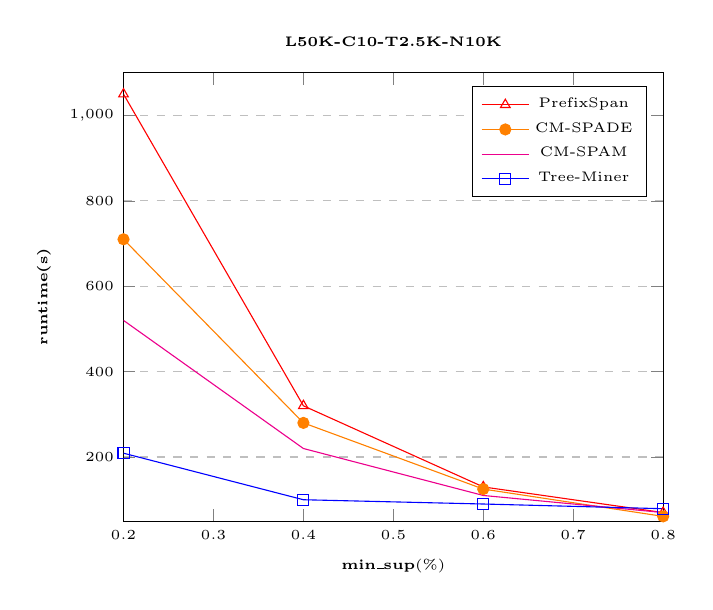
\begin{tikzpicture}
\begin{axis}[
    title={\textbf{L50K-C10-T2.5K-N10K}},
    xlabel={$\textbf{min\_sup}$(\%)},
    ylabel={\textbf{runtime(s)}},
    xmin=0.2, xmax=0.8,
    ymin=50, ymax=1100,
    %xtick={38, 40, 42, 44, 46, 48},
    %ytick={10, 20, 30, 40, 50},
    legend pos=north east,
    ymajorgrids=true,
    grid style=dashed,
   legend style={font=\tiny},
    title style={font=\tiny},
    label style={font=\tiny},
    every tick label/.append style={font=\tiny}
]

\addplot[
    color=red,
    mark=triangle,
    ]
    coordinates {
        (0.8,  70) 
        (0.6, 130)
        (0.4, 320)
        (0.2,  1050)
    };
    \addlegendentry{PrefixSpan}
    
    \addplot[
    color=orange,
    mark=*
    ]
    coordinates {
        (0.8,  61) 
        (0.6, 125)
        (0.4, 280)
        (0.2, 710)
    };
    \addlegendentry{CM-SPADE}

  \addplot[
    color=magenta
    ]
    coordinates {
        (0.8,  70) 
        (0.6, 110)
        (0.4, 220)
        (0.2, 520)
    };
    \addlegendentry{CM-SPAM}
    
   
    \addplot[
    color=blue,
    mark=square,
    ]
    coordinates {
        (0.8,  79) 
        (0.6, 90)
        (0.4, 100)
        (0.2,  209)
    };
    \addlegendentry{Tree-Miner}
\end{axis}
\end{tikzpicture}
        \end{adjustbox}
         \caption{}
        \end{subfigure}
        \begin{subfigure}{.3\linewidth}
            \begin{adjustbox}{max width=\textwidth}
            \centering
           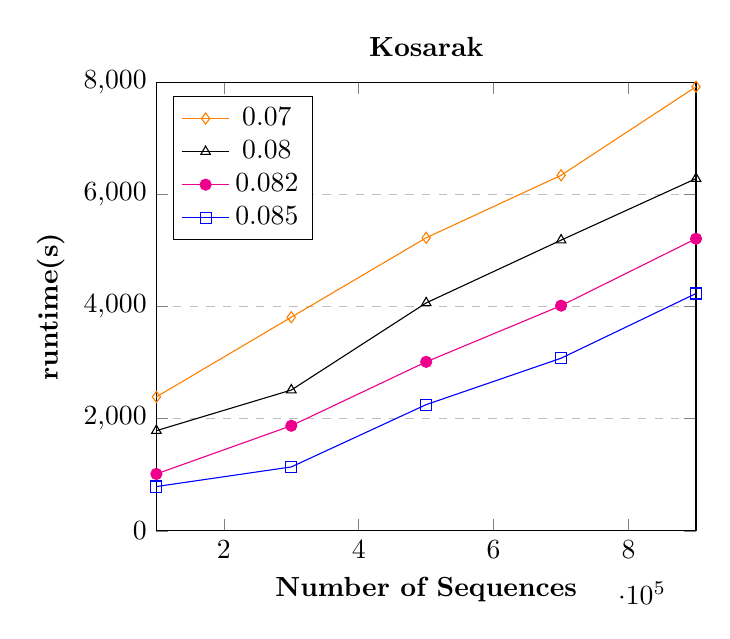
\begin{tikzpicture}
              \begin{axis}[
    title={\textbf{Kosarak}},
    xlabel={\textbf{Number of Sequences}},
    ylabel={\textbf{runtime(s)}},
    xmin=100000, xmax=900000,
    ymin=0, ymax=8000,
    legend pos=north west,
    ymajorgrids=true,
    grid style=dashed,
]
    \addplot[
    color=orange,
    mark=diamond,
    ]
    coordinates {
      (900000,7925)  
      (700000,6344) 
      (500000,5229)
      (300000,3812)
      (100000,2390)
    };
    \addplot[
    color=black,
    mark=triangle
    ]
    coordinates {
      (900000,6285) 
      (700000,5187) 
      (500000,4067)
      (300000,2512)
      (100000,1787)
    };
    \addplot[
    color=magenta,
    mark=*,
    ]
    coordinates {
        (900000,5212)
        (700000,4018) 
        (500000,3015)
        (300000,1875)
        (100000,1015)
    };
    \addplot[
        color=blue,
        mark=square,
        ]
        coordinates {
         (900000,4235) 
         (700000,3080) 
         (500000,2252)
         (300000,1140)
         (100000,790)
        };
    \legend{0.07, 0.08, 0.082, 0.085}   
\end{axis}
           \end{tikzpicture}
           \end{adjustbox}
           \caption{}
           \end{subfigure}
        
        \caption{(a) - (g): Runtime Comparisons, (h) Scalability Comparison for Tree-Miner}
        \label{graph:runtime_scalability_comparison_tree_miner}
        \end{figure*}

\textcolor{blue}{up to now, the comparison has been shown with the base mining approaches as the proposed solution was designed as a new mining algorithm for SPM problem. We have also tried to apply the proposed solution in some different types of SPM problems which are mostly application centric and borrows concepts from base pattern mining techniques.}


\textcolor{blue}{In this regard, we compared our proposal with \cite{he2019significance} and \cite{tarus2018hybrid} two recent literatures. In \cite{he2019significance}, they mined discriminative sequential patterns using significance threshold. Here they first generate all the frequent patterns using GSP, then conduct multi level correlation analysis in such regard. In \cite{tarus2018hybrid}, they designed a context based e-learning recommendation system using the utility of SPM algorithms where GSP was used in such regard. We applied our proposal in these literatures and could directly embed it without any modification. As pattern growth approaches are significantly faster compared to GSP, our Tree-Miner improved the performance of the pattern generation level to a significant amount leading to an overall improvement. Some experimental results have been provided to support the claim in Fig \ref{figure:runtime_with_gsp}. For the comparisons, all the base datasets have been used here, multiple single itemed  sequential events.} 

\textcolor{blue}{In the figure (a) and (b) shows the results of Tree-Miner embedded performance improvement where Disc denotes the applied solution in literature \cite{he2019significance} whereas Tree-Miner with Disc denotes our solution. For the comparison here, significance level ($\alpha$) as per stated in the article is fixed and the support threshold value is varied.}

\textcolor{blue}{Similarly, some results have been shown after comparing with \cite{tarus2018hybrid}. In this article, a recommendation system is built based on context awareness for e-learning purpose. For this purpose, they needed relevant web click stream data, users' knowledge profile and ratings for each resource upon which they calculated the suggestion metrics. To bring the context aware recommendation, they used GSP to filter out the suggestions after generating a set of frequent sequential patterns or web logs visited by the users. Keeping all their contributions align, the comparison comes here is how the pattern generation process can be made faster using our proposal. In Fig. \ref{figure:runtime_with_gsp} (c) and (d), we have shown the performance of GSP with Tree-Miner in two click stream datasets. Here we have used the base datasets, single event with multiple itemed events for the comparison.}         
\begin{figure*}[!tb]
            \centering
        \begin{subfigure}{.24\linewidth}
          \centering
        \begin{adjustbox}{max width=\textwidth}
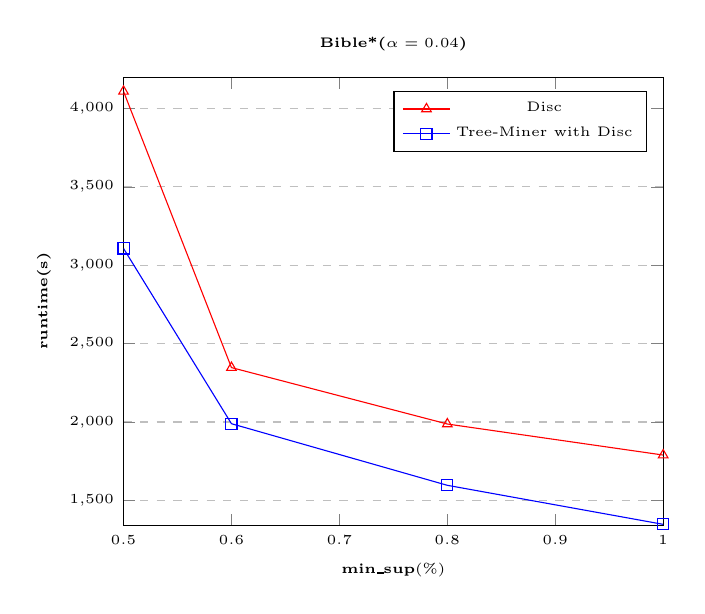
\begin{tikzpicture}
\begin{axis}[
    title={\textbf{Bible*($\alpha=0.04$)}},
    xlabel={$\textbf{min\_sup}$(\%)},
    ylabel={\textbf{runtime(s)}},
    xmin=0.5, xmax=1,
    ymin=1340, ymax=4200,
    %xtick={38, 40, 42, 44, 46, 48},
    %ytick={10, 20, 30, 40, 50},
    legend pos=north east,
    ymajorgrids=true,
    grid style=dashed,
   legend style={font=\tiny},
    title style={font=\tiny},
    label style={font=\tiny},
    every tick label/.append style={font=\tiny}
]

\addplot[
    color=red,
    mark=triangle,
    ]
    coordinates {
        (0.5, 4109) 
        (0.6, 2347)
        (0.8, 1987)
        (1,   1789)
    };
    \addlegendentry{Disc}
    
    \addplot[
    color=blue,
    mark=square,
    ]
    coordinates {
        (0.5, 3107) 
        (0.6, 1989)
        (0.8, 1596)
        (1,   1347)
    };
    \addlegendentry{Tree-Miner with Disc}
\end{axis}
\end{tikzpicture}
        \end{adjustbox}
         \caption{}
        \end{subfigure}
        \begin{subfigure}{.24\linewidth}
          \centering
        \begin{adjustbox}{max width=\textwidth}
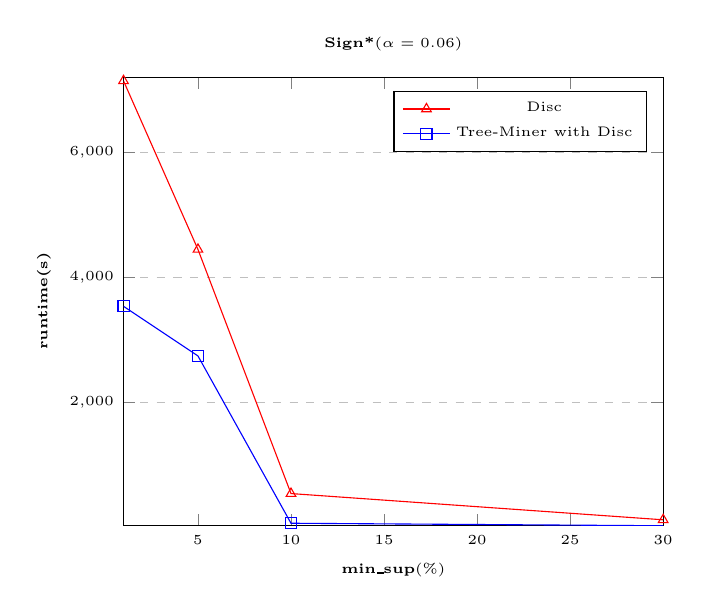
\begin{tikzpicture}
\begin{axis}[
    title={\textbf{Sign*$(\alpha=0.06)$}},
    xlabel={$\textbf{min\_sup}$(\%)},
    ylabel={\textbf{runtime(s)}},
    xmin=1, xmax=30,
    ymin=40, ymax=7200,
    %xtick={38, 40, 42, 44, 46, 48},
    %ytick={10, 20, 30, 40, 50},
    legend pos=north east,
    ymajorgrids=true,
    grid style=dashed,
    legend style={font=\tiny},
    title style={font=\tiny},
    label style={font=\tiny},
    every tick label/.append style={font=\tiny}
]

\addplot[
    color=red,
    mark=triangle,
    ]
    coordinates {
        (30,130) 
        (10, 549)
        (5, 4448)
        (1, 7140)
    };
    \addlegendentry{Disc}
    
    \addplot[
    color=blue,
    mark=square,
    ]
    coordinates {
        (30,35) 
        (10, 75)
        (5, 2747)
        (1, 3540)
    };
    \addlegendentry{Tree-Miner with Disc}
\end{axis}
\end{tikzpicture}
        \end{adjustbox}
        \caption{}
        \end{subfigure}
        \begin{subfigure}{.24\linewidth}
          \centering
        \begin{adjustbox}{max width=\textwidth}
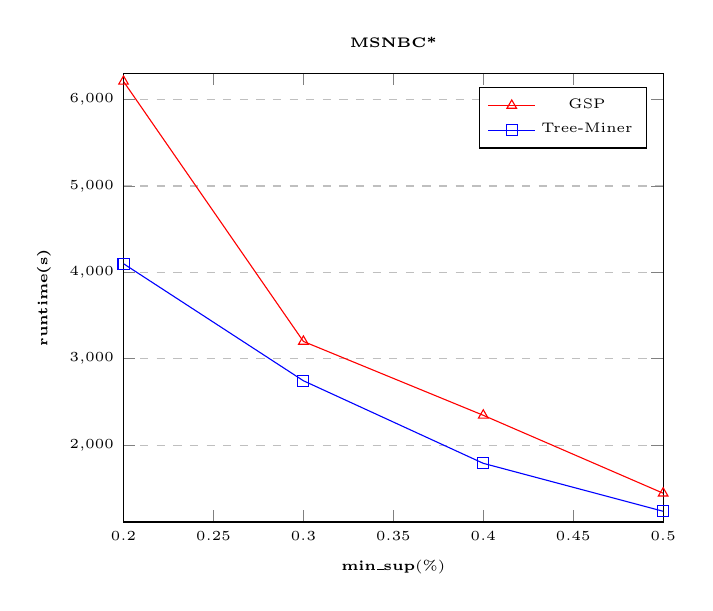
\begin{tikzpicture}
\begin{axis}[
    title={\textbf{MSNBC*}},
    xlabel={$\textbf{min\_sup}$(\%)},
    ylabel={\textbf{runtime(s)}},
    xmin=0.2, xmax=0.5,
    ymin=1110, ymax=6300,
    %xtick={38, 40, 42, 44, 46, 48},
    %ytick={10, 20, 30, 40, 50},
    legend pos=north east,
    ymajorgrids=true,
    grid style=dashed,
    legend style={font=\tiny},
    title style={font=\tiny},
    label style={font=\tiny},
    every tick label/.append style={font=\tiny}
]

\addplot[
    color=red,
    mark=triangle,
    ]
    coordinates {
        (0.5, 1443) 
        (0.4, 2345)
        (0.3, 3200)
        (0.2,  6210)
    };
    \addlegendentry{GSP}
    
    \addplot[
    color=blue,
    mark=square,
    ]
    coordinates {
        (0.5,  1234) 
        (0.4, 1789)
        (0.3, 2745)
        (0.2,  4100)
    };
    \addlegendentry{Tree-Miner}
\end{axis}
\end{tikzpicture}
        \end{adjustbox}
        \caption{}
        \end{subfigure}
        \begin{subfigure}{.24\linewidth}
          \centering
        \begin{adjustbox}{max width=\textwidth}
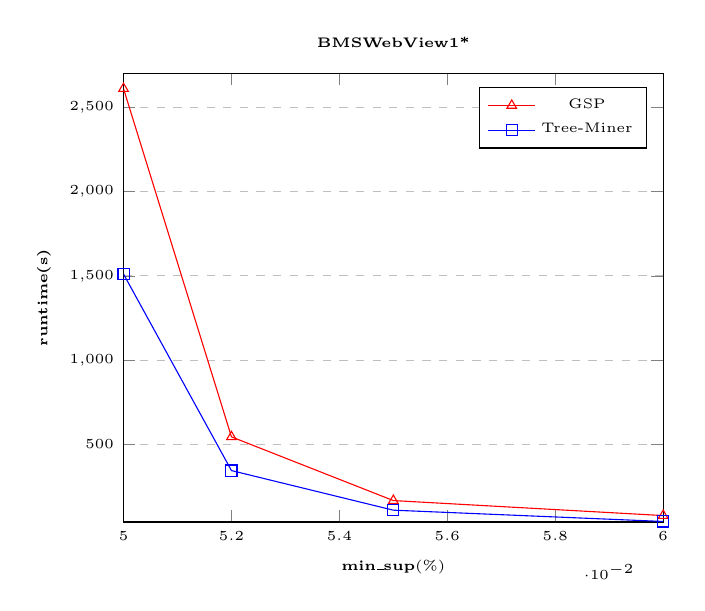
\begin{tikzpicture}
\begin{axis}[
    title={\textbf{BMSWebView1*}},
    xlabel={$\textbf{min\_sup}$(\%)},
    ylabel={\textbf{runtime(s)}},
    xmin=0.05, xmax=0.06,
    ymin=40, ymax=2700,
    %xtick={38, 40, 42, 44, 46, 48},
    %ytick={10, 20, 30, 40, 50},
    legend pos=north east,
    ymajorgrids=true,
    grid style=dashed,
    legend style={font=\tiny},
    title style={font=\tiny},
    label style={font=\tiny},
    every tick label/.append style={font=\tiny}
]

\addplot[
    color=red,
    mark=triangle,
    ]
    coordinates {
        (0.06,  78) 
        (0.055, 167)
        (0.052, 545)
        (0.05,  2611)
    };
    \addlegendentry{GSP}
    
    \addplot[
    color=blue,
    mark=square,
    ]
    coordinates {
        (0.06,  43) 
        (0.055, 110)
        (0.052, 345)
        (0.05,  1511)
    };
    \addlegendentry{Tree-Miner}
\end{axis}
\end{tikzpicture}
        \end{adjustbox}
        \caption{}
        \end{subfigure}
        \caption{\textcolor{blue}{Runtime Improvement using Tree-Miner over GSP based literature}}
        \label{figure:runtime_with_gsp}
        \end{figure*}

\textcolor{blue}{We have also compared our solution to \cite{hosseininasab2019constraint}, a novel Mining with Decision Diagram (MDD) based approach to solve constraint-based sequential pattern mining. But to make a fair comparison with the literature's solution, we had to modify our algorithm and datasets to some extent. A summary of such modifications are shown as below,} 

\textcolor{blue}{\begin{itemize}
    \item In the literature, how multiple itemed event will be handled was not proposed. So, for the comparisons, all the base datasets have been used here, multiple single itemed  sequential events.  
    \item The literature constructed their proposed MDD nodes over an initially given support threshold value by pruning nodes. This idea can easily be embedded in our solution as ours is more generic. When the next links are calculated, we can apply the breadth-first and upper bound based pattern generation concept to reduce many next link connection.\\ 
    For example, we want to generate $\alpha \,\to\, \alpha\beta$. Here $N_{\alpha}=\{2, 3, 4\}$, $S_{\alpha}=9$, $C(2)=C(3)=C(4)=3$, $\delta=8$. We want to calculate next links for $\beta$ from each $v\in N_{\alpha}$. Let from $2$ we need to make a next link connection with $5$ for $\beta$ where $C(5)=1$. So using breadth-first technique, we can see $S_{\alpha\beta}=9-3+1<\delta$. Thus we can stop constructing all the next links for $\alpha \,\to \, \beta$ and its super patterns for all the remaining nodes along with pruning this pattern from the generation. 
    \item Two solutions' comparisons are done only over support threshold constraint. The result is shown in Fig. \ref{graph:runtime_comparison_with_mdd}. 
\end{itemize}}

\begin{figure*}[!tb]
            \centering
        \begin{subfigure}{.3\linewidth}
          \centering
        \begin{adjustbox}{max width=\textwidth}
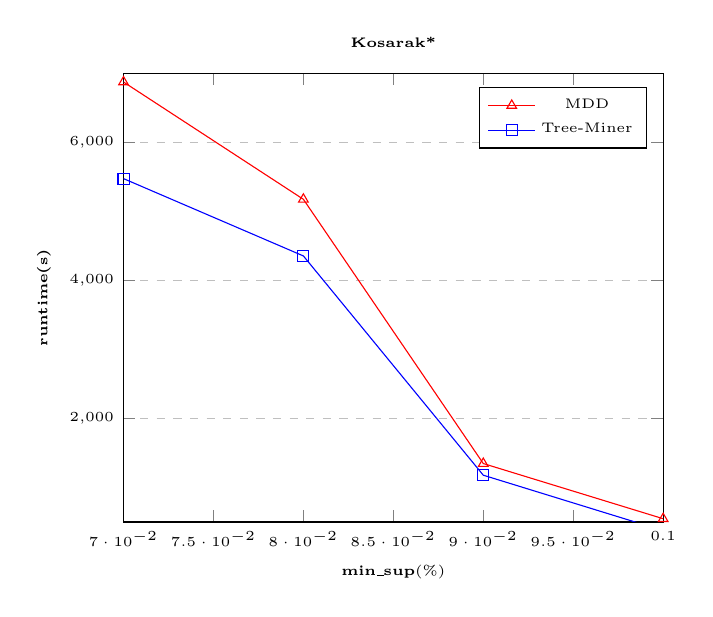
\begin{tikzpicture}
\begin{axis}[
    title={\textbf{Kosarak*}},
    xlabel={$\textbf{min\_sup}$(\%)},
    ylabel={\textbf{runtime(s)}},
    xmin=0.07, xmax=0.1,
    ymin=500, ymax=7000,
    %xtick={38, 40, 42, 44, 46, 48},
    %ytick={10, 20, 30, 40, 50},
    legend pos=north east,
    ymajorgrids=true,
    grid style=dashed,
   legend style={font=\tiny},
    title style={font=\tiny},
    label style={font=\tiny},
    every tick label/.append style={font=\tiny}
]

\addplot[
    color=red,
    mark=triangle,
    ]
    coordinates {
        (0.1,547)
        (0.09,1347)
        (0.08,5178)
        (0.07,6879)
    };
    \addlegendentry{MDD}
    
    \addplot[
    color=blue,
    mark=square,
    ]
    coordinates {
        (0.1,374)
        (0.09,1178)
        (0.08,4357)
        (0.07,5478)
    };
    \addlegendentry{Tree-Miner}
\end{axis}
\end{tikzpicture}
        \end{adjustbox}
         \caption{}
        \end{subfigure}
        \begin{subfigure}{.3\linewidth}
          \centering
        \begin{adjustbox}{max width=\textwidth}
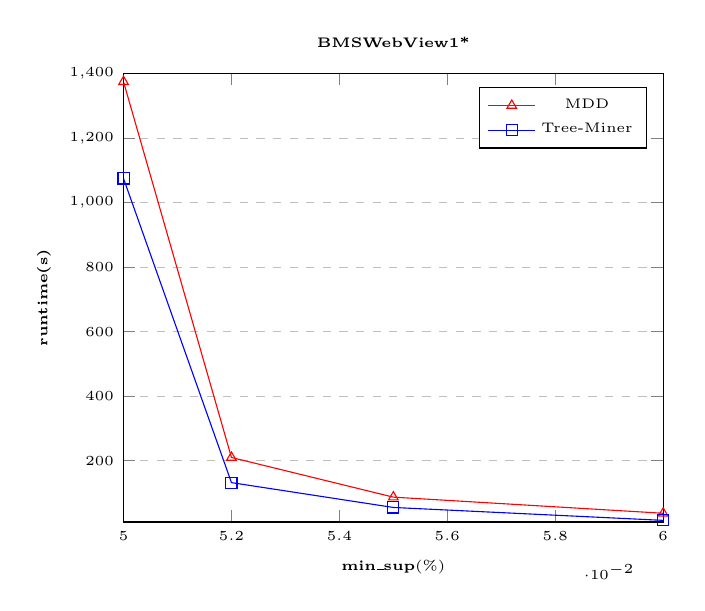
\begin{tikzpicture}
\begin{axis}[
    title={\textbf{BMSWebView1*}},
    xlabel={$\textbf{min\_sup}$(\%)},
    ylabel={\textbf{runtime(s)}},
    xmin=0.05, xmax=0.06,
    ymin=10, ymax=1400,
    %xtick={38, 40, 42, 44, 46, 48},
    %ytick={10, 20, 30, 40, 50},
    legend pos=north east,
    ymajorgrids=true,
    grid style=dashed,
    legend style={font=\tiny},
    title style={font=\tiny},
    label style={font=\tiny},
    every tick label/.append style={font=\tiny}
]

\addplot[
    color=red,
    mark=triangle,
    ]
    coordinates {
      (0.06,  37) 
        (0.055, 87)
        (0.052, 210)
        (0.05,  1375)
    };
    \addlegendentry{MDD}
    
    \addplot[
    color=blue,
    mark=square,
    ]
    coordinates {
        (0.06,  15) 
        (0.055, 55)
        (0.052, 132)
        (0.05,  1075)
    };
    \addlegendentry{Tree-Miner}
\end{axis}
\end{tikzpicture}
        \end{adjustbox}
        \caption{}
        \end{subfigure}
        \begin{subfigure}{.3\linewidth}
          \centering
        \begin{adjustbox}{max width=\textwidth}
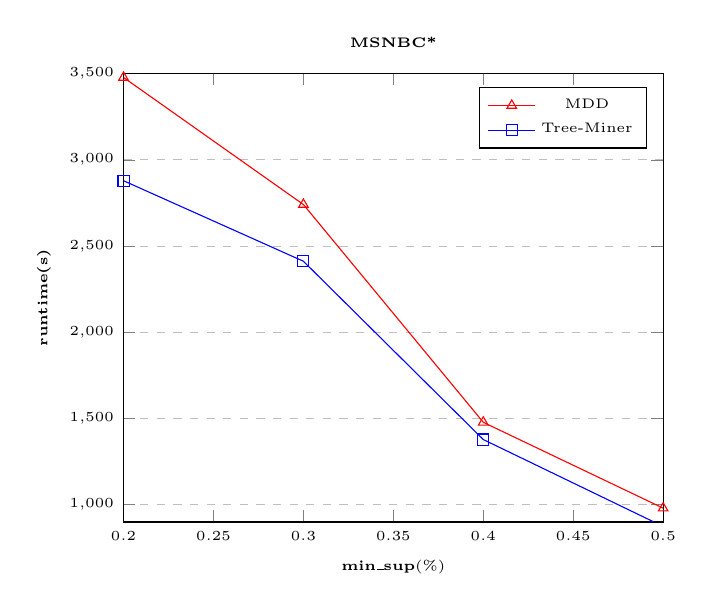
\begin{tikzpicture}
\begin{axis}[
    title={\textbf{MSNBC*}},
    xlabel={$\textbf{min\_sup}$(\%)},
    ylabel={\textbf{runtime(s)}},
    xmin=0.2, xmax=0.5,
    ymin=900, ymax=3500,
    %xtick={38, 40, 42, 44, 46, 48},
    %ytick={10, 20, 30, 40, 50},
    legend pos=north east,
    ymajorgrids=true,
    grid style=dashed,
    legend style={font=\tiny},
    title style={font=\tiny},
    label style={font=\tiny},
    every tick label/.append style={font=\tiny}
]

\addplot[
    color=red,
    mark=triangle,
    ]
    coordinates {
        (0.5, 980) 
        (0.4, 1478)
        (0.3, 2741)
        (0.2, 3478)
    };
    \addlegendentry{MDD}
    
    \addplot[
    color=blue,
    mark=square,
    ]
    coordinates {
        (0.5,  874) 
        (0.4, 1378)
        (0.3, 2412)
        (0.2,  2879)
    };
    \addlegendentry{Tree-Miner}
\end{axis}
\end{tikzpicture}
        \end{adjustbox}
        \caption{}
        \end{subfigure}
        \caption{\textcolor{blue}{Runtime Comparisons between Tree-Miner and MDD}}
        \label{graph:runtime_comparison_with_mdd}
        \end{figure*}

\textcolor{blue}{From the figures, it can be observed that Tree-Miner with SP-Tree performs comparatively better. The main reasons lie in its larger flexibility, e.g., multiple event handling, easily modifiable, bit based usage advantages, etc and pruning strategies. The results for Kosarak, MSNBC and BMSWebView1 have been shown in the figure. As previously stated, using next links we can perform faster jumps in the database along with using the rich pruning techniques a good amount of pattern searching can be omitted.}  


Due to the structured representation of the information, our solution needs comparatively more memory. We maintain SP-Tree and co-occurrence information which gives control over the database and helps significantly during pattern extension. Prefixspan uses database projection technique, CM-SPADE uses lattice alike structures and CM-SPAM uses bit based array structures to perform projection and calculate the support of a pattern. During pattern extension, the compared algorithms create and maintain some sort of additional supporting structures in runtime whereas our proposed solution uses the base tree structures' nodes for this purpose. Through some additional memory usage, we gain significant amount of improvement in mining which we will show shortly and considering the runtime improvement this should be tolerable. We present an analysis in Fig. \ref{graph:memory_comparison_tree_miner} for two datasets. From the figure, it can be seen that our solution comparatively needs some additional memory and we have already discussed the underlying reasoning behind it. The difference will be comparatively closer in denser datasets due to tree's node overlapping characteristics.  

We have also conducted a scalability analysis of Tree-Miner and presented the result in Fig. \ref{graph:runtime_scalability_comparison_tree_miner} (g) experimenting over the lage \textit{Kosarak} dataset. We started with 100000 transactions, gradually increased it and recorded the performance for various $min\_sup$. The corresponding figure shows the linear scalability of the solution. Another important concern can be, as our solution is based on defined structures, do their construction times create any bottleneck during mining. For this purpose we present an analysis in Table \ref{table:construction_time_tree_miner} where we can see that, the total construction time is quite insignificant compared to the total mining time and does not create bottleneck. In the last three columns of Table \ref{table:construction_time_tree_miner} we have also shown the corresponding runtime performance improvement in mining over the comparing algorithms ($Pr$: PrefixSpan, $SP$: CM-SPADE, $SM$: CM-SPAM). This basically states the significance of how much we can improve mining performance with very small time cost in pre-processing.



\begin{figure*}[!tb]
            \centering
        \begin{subfigure}{0.4\linewidth}
\centering
 \begin{adjustbox}{max width=\textwidth}
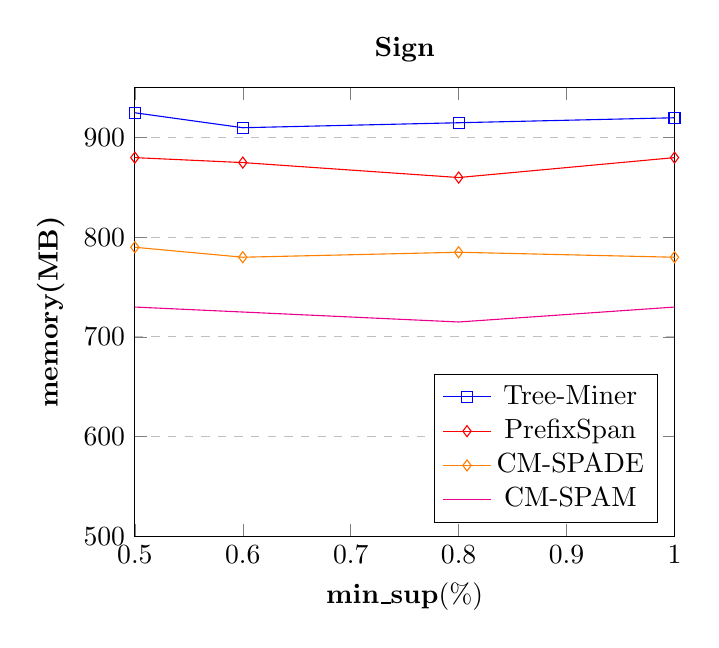
\begin{tikzpicture}
\begin{axis}[
    title={\textbf{Sign}},
    xlabel={$\textbf{min\_sup}$(\%)},
    ylabel={\textbf{memory(MB)}},
    xmin=0.5, xmax=1,
    ymin=500, ymax=950,
    %xtick={1200, 1500, 2000},
    %ytick={0,2,4,6,8},
    legend pos=south east,
    ymajorgrids=true,
    grid style=dashed,
]

%(41, 12)
%(47, 9)
%(55, 7)

%tree-miner
\addplot[
    color=blue,
    mark=square,
    ]
    coordinates {
        (0.5, 925) 
        (0.6, 910)
        (0.8, 915)
        (1, 920)
    };
    \addlegendentry{Tree-Miner}

  \addplot[
    color=red,
    mark=diamond,
    ]
    coordinates {
        (0.5, 880) 
        (0.6, 875)
        (0.8, 860)
        (1, 880)
    };
    \addlegendentry{PrefixSpan}

\addplot[
    color=orange,
    mark=diamond,
    ]
    coordinates {
        (0.5, 790) 
        (0.6, 780)
        (0.8, 785)
        (1, 780)
    };
    \addlegendentry{CM-SPADE}
    
    \addplot[
    color=magenta
    ]
    coordinates {
        (0.5, 730) 
        (0.6, 725)
        (0.8, 715)
        (1, 730)
    };
    \addlegendentry{CM-SPAM}
    
\end{axis}
\end{tikzpicture}
\end{adjustbox}
\caption{}
\end{subfigure}
        \begin{subfigure}{0.4\linewidth}
\centering
 \begin{adjustbox}{max width=\textwidth}
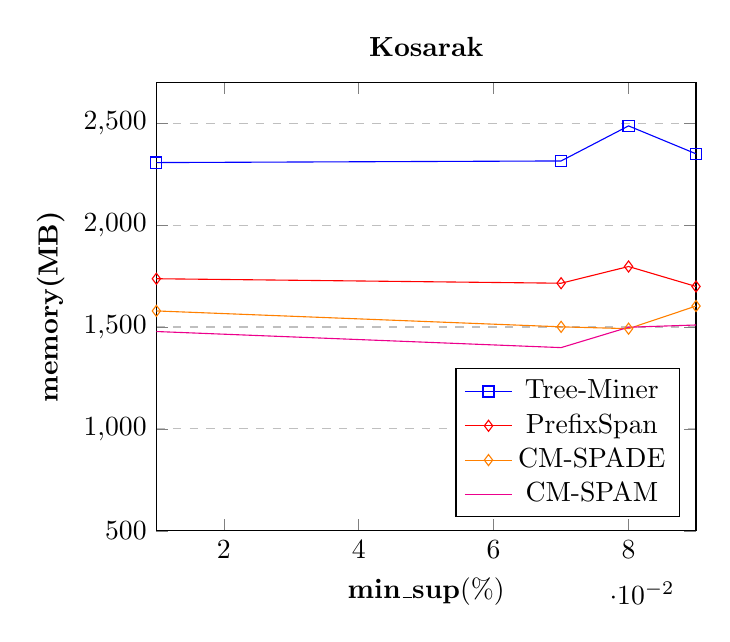
\begin{tikzpicture}
\begin{axis}[
    title={\textbf{Kosarak}},
    xlabel={$\textbf{min\_sup}$(\%)},
    ylabel={\textbf{memory(MB)}},
    xmin=0.01, xmax=0.09,
    ymin=500, ymax=2700,
    %xtick={1200, 1500, 2000},
    %ytick={0,2,4,6,8},
    legend pos=south east,
    ymajorgrids=true,
    grid style=dashed,
]

%(41, 12)
%(47, 9)
%(55, 7)

%tree-miner
\addplot[
    color=blue,
    mark=square,
    ]
    coordinates {
        (0.01, 2307)
        (0.07, 2315)
        (0.08, 2487)
        (0.09, 2350)
    };
    \addlegendentry{Tree-Miner}

  \addplot[
    color=red,
    mark=diamond,
    ]
    coordinates {
        (0.01, 1737)
        (0.07, 1715)
        (0.08, 1797)
        (0.09, 1699)
    };
    \addlegendentry{PrefixSpan}

    \addplot[
        color=orange,
        mark=diamond,
        ]
        coordinates {
            (0.01, 1579) 
            (0.07, 1501)
            (0.08, 1492)
            (0.09, 1603)
        };
        \addlegendentry{CM-SPADE}
    
    \addplot[
    color=magenta
    ]
    coordinates {
        (0.01, 1478) 
        (0.07, 1399)
        (0.08, 1499)
        (0.09, 1510)
    };
    \addlegendentry{CM-SPAM}
    
\end{axis}
\end{tikzpicture}
\end{adjustbox}
\caption{}
\end{subfigure}
        \caption{Memory Comparisons for Tree-Miner}
        \label{graph:memory_comparison_tree_miner}
        \end{figure*}

\begin{table*}[!htbp]
\centering
%% increase table row spacing, adjust to taste
%\renewcommand{\arraystretch}{1.3}
% if using array.sty, it might be a good idea to tweak the value of
% \extrarowheight as needed to properly center the text within the cells
%\centering
%% Some packages, such as MDW tools, offer better commands for making tables
%% than the plain LaTeX2e tabular which is used here.
\begin{tabular}{|l|l|l|l|l|l|l|l|}
\hline
Dataset & Construct- & Mining & $min\_sup$ & $\frac{C}{M}$ & $ M $ & $M$ & $M$ \\ 
& ion Time  &  Time & (\%) & (\%) & vs & vs & vs\\
& (Sec.) & (Sec.) & & & $Pr$ & $SP$ & $SM$\\ 
& ($C$) &  ($M$) & & & (\%) & (\%)&(\%)\\ 
\hline
 Bible & 40 & 2907 & 0.5 & 1.3 & 29  & 20 & 26\\ \hline
 BMSWebView1 & 5 & 1321 &  0.05 & 0.3 & 64 & 52 & 45\\ \hline
 Sign  &  16  &  2448 & 1 & 0.6 & 48 & 28 & 40\\ \hline
 MSNBC & 14 & 3700 & 0.2 & 0.3 & 33 & 18 & 24\\ \hline
 Kosarak & 130 & 7925 & 0.07 & 1.6 & 29 & 22 & 15\\ \hline
L20-C10-T5-N1K & 10 & 1012 & 0.025 & 1 & 56 & 17 & 33\\ \hline
L50-C10-T2.5-N10K & 20 & 2010 & 0.02 & 0.9 & 76 & 64 & 54\\ \hline
\end{tabular}
\caption{Construction Time Vs Mining Time}
\label{table:construction_time_tree_miner}
\end{table*}




\subsection{IncTree-Miner}
In this section, we will analyze the performance of IncTree-Miner based on various metrics.

\subsubsection{Runtime, Memory Usage, Scalability}
Our IncTree-Miner contains all the novelty of Tree-Miner and designs a set of concepts to implicitly track the incremental database which ultimately helps to efficiently mine those patterns which are affected due to the addition of incremental database. It separates the modified and unmodified subtrees, performs projection separately and combines the results to provide the final output. Using modified next links and support count attributes we efficiently detect the modified subtrees and the updated patterns with their changed support. During pattern extensions, first we project in the incremental database and from there using \textit{infrequent to frequent} transition property we first detect which infrequent patterns have chance to be frequent and then decide to perform projection in the remaining database for them. This approach also helps to efficiently update the frequency of the existing frequent patterns which are affected due to the incremental database also leading to the detection of the previously frequent and currently infrequent patterns. We also use BPFSP-Tree as pattern storage which keeps the projection information of the patterns using IncSP-Tree nodes. It reduces the number of DB scans and efficiently removes the infrequent patterns using the bottom-up strategy. It also maintains NIB buffer which makes use of the cost to calculate the support of an infrequent pattern by giving an idea regarding previous support during the following iterations. Sequence Summarizer also helps to incrementally update the co-occurrence information.


In Fig. \ref{graph:runtime_scalability_comparison_inc_tree_miner} (a)-(g), we have shown the runtime performance of IncTree-Miner with $PBIncSpan$ and $IncSP$. From the figure, it is obvious that our proposed algorithm improves runtime by a significant amount. IncSP is based on candidate generation and testing paradigm and it is bound to be slow compared to pattern growth algorithms. PBIncSapn is an efficient solution that follows the pattern growth approach along with applying two efficient pruning mechanisms, width and depth pruning. But these are basically a subset of pruning mechanisms we maintain. PBIncSpan saves the projection information using pseudo projections of the database to reduce the DB scan, whereas we use the compact IncSP-Tree node pointers based BPFSP-Tree for this purpose. Similar to Tree-Miner our performance improvement is quite visible at lower thresholds. As the number of patterns (both frequent and updated) is very small at higher thresholds, the improvement is not much differentiable.

\begin{figure*}[!tb]
        \centering
         \begin{subfigure}{.3\linewidth}
          \centering
           \begin{adjustbox}{max width=\textwidth}
           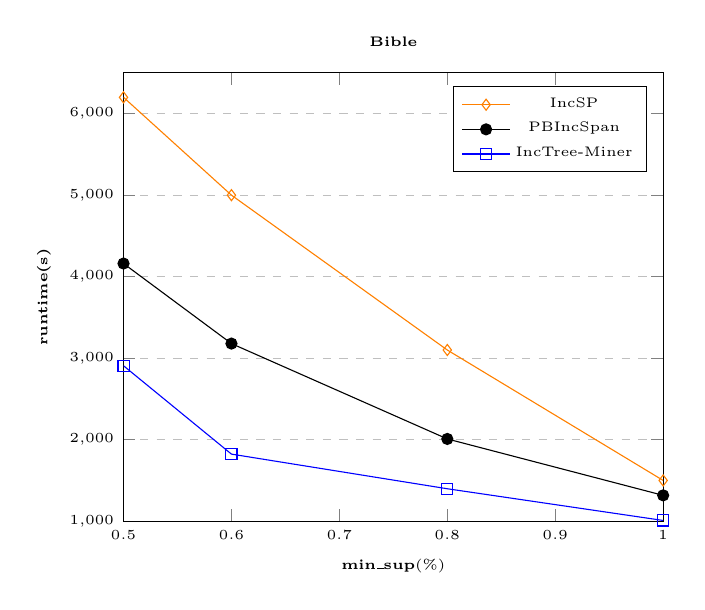
\begin{tikzpicture}
              \begin{axis}[
    title={\textbf{Bible}},
    xlabel={$\textbf{min\_sup}(\%)$},
    ylabel={\textbf{runtime(s)}},
    xmin=0.5, xmax=1,
    ymin=1000, ymax=6500,
    legend pos=north east,
    ymajorgrids=true,
    grid style=dashed,
    legend style={font=\tiny},
    title style={font=\tiny},
    label style={font=\tiny},
    every tick label/.append style={font=\tiny}
]

% (70, 2456.14 * 2.5 = 6140.25)
% (80, 1331.05 * 2.2 = 2928.31)
% (90, 722.725 * 1.8 = 1300.905)
%prefixspan

   \addplot[
    color=orange,
    mark=diamond,
    ]
    coordinates {
        (0.5, 6200) 
        (0.6, 5000)
        (0.8, 3100)
        (1, 1500)  
    };
   
   \addlegendentry{IncSP};
  
   \addplot[
    color=black,
    mark=*,
    ]
    coordinates {
        (0.5, 4161) 
        (0.6, 3179)
        (0.8, 2009)
        (1, 1317)
    };
   \addlegendentry{PBIncSpan};
   
    \addplot[
        color=blue,
        mark=square,
        ]
        coordinates {
            (0.5, 2907) 
            (0.6, 1823)
            (0.8, 1398)
            (1,   1009)
        };
   \addlegendentry{IncTree-Miner};
\end{axis}
           \end{tikzpicture}
          \end{adjustbox}
          \caption{}
         \end{subfigure}
        \begin{subfigure}{.3\linewidth}
          \centering
           \begin{adjustbox}{max width=\textwidth}
           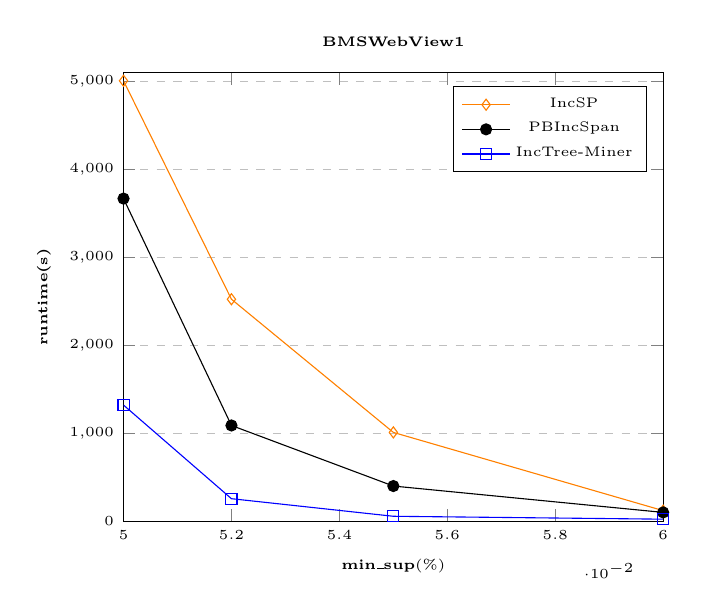
\begin{tikzpicture}
              \begin{axis}[
    title={\textbf{BMSWebView1}},
     xlabel={$\textbf{min\_sup}(\%)$},
    ylabel={\textbf{runtime(s)}},
    xmin=0.05, xmax=0.06,
    ymin=0, ymax=5100,
    legend pos=north east,
    ymajorgrids=true,
    grid style=dashed,
    legend style={font=\tiny},
    title style={font=\tiny},
    label style={font=\tiny},
    every tick label/.append style={font=\tiny}
]
    \addplot[
    color=orange,
    mark=diamond,
    ]
    coordinates {
            (0.06,  120) 
            (0.055, 1010)
            (0.052, 2525)
            (0.05,  5010)
    };
    \addlegendentry{IncSP};
    
   
    \addplot[
    color=black,
    mark=*,
    ]
    coordinates {
            (0.06,  100) 
            (0.055, 400)
            (0.052, 1089)
            (0.05,  3670)
    };
    
    \addlegendentry{PBIncSpan};
     
    %tree-miner
    \addplot[
        color=blue,
        mark=square,
        ]
        coordinates {
            (0.06,  23) 
            (0.055, 56)
            (0.052, 256)
            (0.05,  1321)
        };
    \addlegendentry{IncTree-Miner};
\end{axis}
           \end{tikzpicture}
          \end{adjustbox}
          \caption{}
         \end{subfigure}
        \begin{subfigure}{.3\linewidth}
          \centering
           \begin{adjustbox}{max width=\textwidth}
           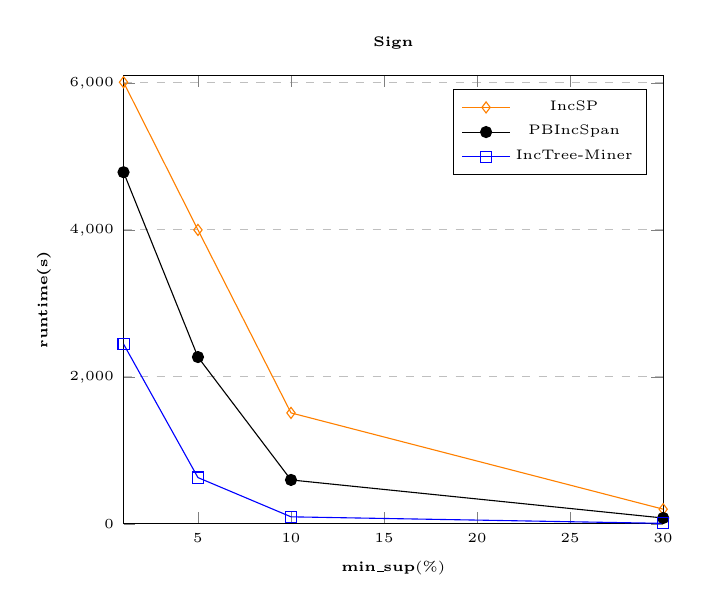
\begin{tikzpicture}
              \begin{axis}[
    title={\textbf{Sign}},
     xlabel={$\textbf{min\_sup}(\%)$},
    ylabel={\textbf{runtime(s)}},
    xmin=1, xmax=30,
    ymin=0, ymax=6100,
    legend pos=north east,
    ymajorgrids=true,
    grid style=dashed,
    legend style={font=\tiny},
    title style={font=\tiny},
    label style={font=\tiny},
    every tick label/.append style={font=\tiny}
]
    \addplot[
    color=orange,
    mark=diamond,
    ]
    coordinates {
            (30, 200) 
            (10, 1510)
            (5, 4000)
            (1, 6010)
    };
    \addlegendentry{IncSP}
    
   
    \addplot[
    color=black,
    mark=*,
    ]
    coordinates {
            (30, 80) 
            (10, 598)
            (5, 2270)
            (1, 4785)
    };
    \addlegendentry{PBIncSpan}
    \addplot[
        color=blue,
        mark=square,
        ]
        coordinates {
            (30, 7) 
            (10, 96)
            (5, 630)
            (1, 2448)
        };
   \addlegendentry{IncTree-Miner}
\end{axis}
           \end{tikzpicture}
          \end{adjustbox}
          \caption{}
         \end{subfigure}
        \begin{subfigure}{.3\linewidth}
          \centering
           \begin{adjustbox}{max width=\textwidth}
           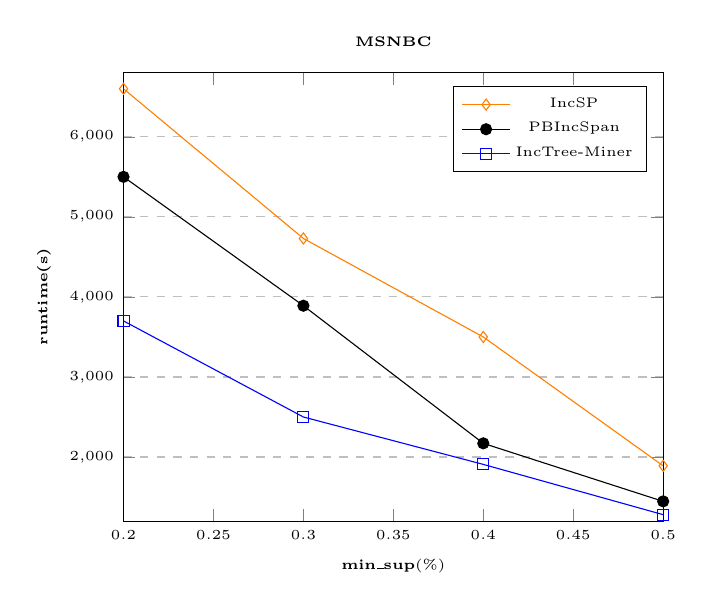
\begin{tikzpicture}
              \begin{axis}[
    title={\textbf{MSNBC}},
    xlabel={$\textbf{min\_sup}(\%)$},
    ylabel={\textbf{runtime(s)}},
    xmin=0.2, xmax=0.5,
    ymin=1200, ymax=6800,
    legend pos=north east,
    ymajorgrids=true,
    grid style=dashed,
    legend style={font=\tiny},
    title style={font=\tiny},
    label style={font=\tiny},
    every tick label/.append style={font=\tiny}
]
    \addplot[
    color=orange,
    mark=diamond,
    ]
    coordinates {
       (0.5, 1890)
       (0.4, 3500)
       (0.3,4730)
       (0.2,6600)
    };
    \addlegendentry{IncSP}
    
    \addplot[
    color=black,
    mark=*,
    ]
    coordinates {
       (0.5, 1446)
       (0.4, 2171)
       (0.3,3890)
       (0.2,5500)
    };
    \addlegendentry{PBIncSpan}
    %tree-miner
    \addplot[
        color=blue,
        mark=square,
        ]
        coordinates {
            (0.5,1280)
            (0.4,1908)
            (0.3,2500)
            (0.2,3700)
        };
   \addlegendentry{IncTree-Miner}
\end{axis}
           \end{tikzpicture}
          \end{adjustbox}
          \caption{}
         \end{subfigure}
        \begin{subfigure}{.3\linewidth}
          \centering
           \begin{adjustbox}{max width=\textwidth}
           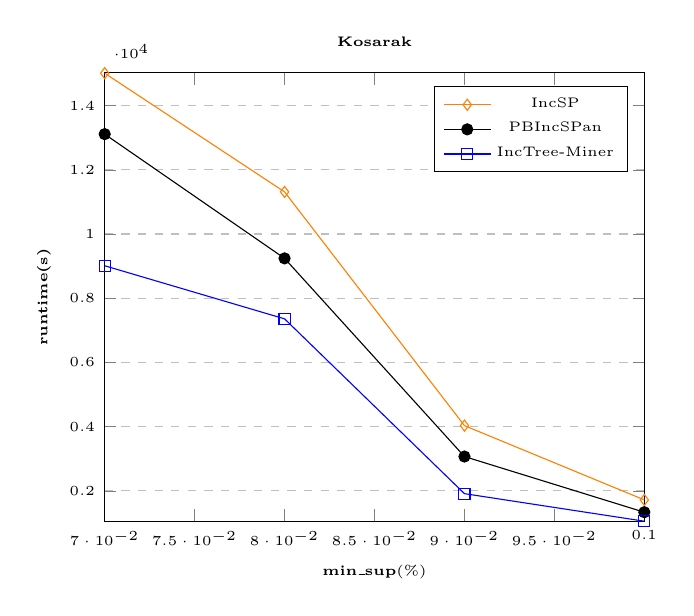
\begin{tikzpicture}
              \begin{axis}[
    title={\textbf{Kosarak}},
     xlabel={$\textbf{min\_sup}(\%)$},
    ylabel={\textbf{runtime(s)}},
    xmin=0.07, xmax=0.1,
    ymin=1055, ymax=15020,
    legend pos=north east,
    ymajorgrids=true,
    grid style=dashed,
    legend style={font=\tiny},
    title style={font=\tiny},
    label style={font=\tiny},
    every tick label/.append style={font=\tiny}
]
    \addplot[
    color=orange,
    mark=diamond,
    ]
    coordinates {
            (0.1, 1718) 
            (0.09, 4032)
            (0.08, 11312)
            (0.07, 15010)
    };
    \addlegendentry{IncSP}
    
    \addplot[
    color=black,
    mark=*,
    ]
    coordinates {
            (0.1, 1335) 
            (0.09, 3069)
            (0.08, 9242)
            (0.07, 13112)
    };
    \addlegendentry{PBIncSPan}
    
    \addplot[
        color=blue,
        mark=square,
        ]
        coordinates {
            (0.1, 1055) 
            (0.09, 1913)
            (0.08, 7358)
            (0.07, 9012)
        };
    \addlegendentry{IncTree-Miner}  
\end{axis}
           \end{tikzpicture}
          \end{adjustbox}
          \caption{}
         \end{subfigure}
       \begin{subfigure}{.3\linewidth}
          \centering
           \begin{adjustbox}{max width=\textwidth}
           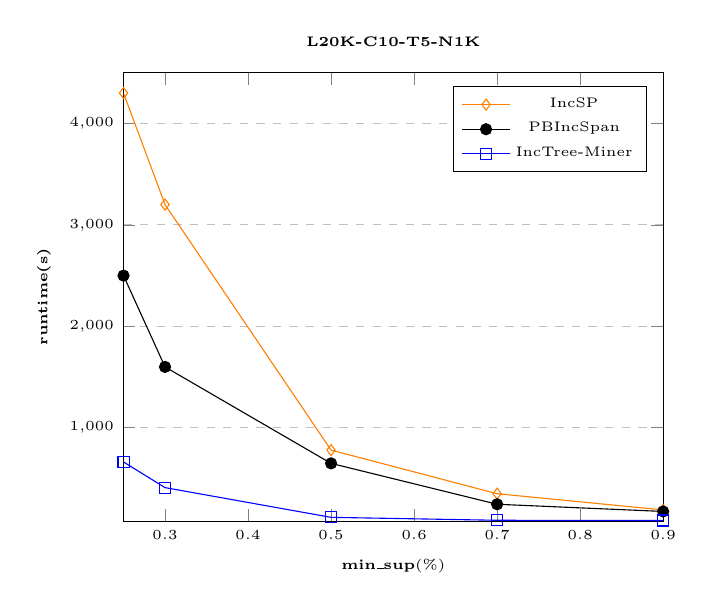
\begin{tikzpicture}
              \begin{axis}[
    title={\textbf{L20K-C10-T5-N1K}},
     xlabel={$\textbf{min\_sup}(\%)$},
    ylabel={\textbf{runtime(s)}},
    xmin=0.25, xmax=0.9,
    ymin=80, ymax=4500,
    legend pos=north east,
    ymajorgrids=true,
    grid style=dashed,
    legend style={font=\tiny},
    title style={font=\tiny},
    label style={font=\tiny},
    every tick label/.append style={font=\tiny}
]

\addplot[
    color=orange,
    mark=diamond,
    ]
    coordinates {
            (0.9, 190) 
            (0.7, 350)
            (0.5, 780)
            (0.3, 3200)
            (0.25, 4300)
    };
    \addlegendentry{IncSP}

    \addplot[
    color=black,
    mark=*,
    ]
    coordinates {
            (0.9, 175) 
            (0.7, 246)
            (0.5, 649)
            (0.3,  1600)
            (0.25, 2500)
    };
    \addlegendentry{PBIncSpan}
     
    %tree-miner
    \addplot[
        color=blue,
        mark=square,
        ]
        coordinates {
            (0.9, 86) 
            (0.7, 88)
            (0.5, 117)
            (0.3,  410)
            (0.25, 663)
        };
   \addlegendentry{IncTree-Miner}
\end{axis}
           \end{tikzpicture}
          \end{adjustbox}
          \caption{}
         \end{subfigure}
      \begin{subfigure}{.3\linewidth}
          \centering
           \begin{adjustbox}{max width=\textwidth}
           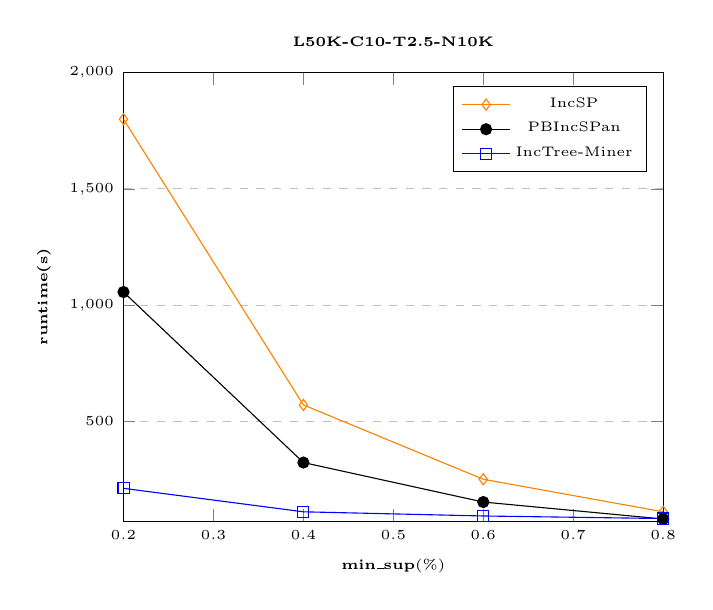
\begin{tikzpicture}
              \begin{axis}[
    title={\textbf{L50K-C10-T2.5-N10K}},
     xlabel={$\textbf{min\_sup}(\%)$},
    ylabel={\textbf{runtime(s)}},
    xmin=0.2, xmax=0.8,
    ymin=70, ymax=2000,
    legend pos=north east,
    ymajorgrids=true,
    grid style=dashed,
    legend style={font=\tiny},
    title style={font=\tiny},
    label style={font=\tiny},
    every tick label/.append style={font=\tiny}
]
    \addplot[
    color=orange,
    mark=diamond,
    ]
    coordinates {
        (0.8, 110) 
        (0.6, 250)
        (0.4, 570)
        (0.2, 1800)
    };
    \addlegendentry{IncSP}
    
    \addplot[
    color=black,
    mark=*,
    ]
    coordinates {
            (0.8, 79) 
            (0.6, 152)
            (0.4, 322)
            (0.2,  1056)
    };
    \addlegendentry{PBIncSPan}
    
    \addplot[
        color=blue,
        mark=square,
        ]
        coordinates {
            (0.8, 81) 
            (0.6, 92)
            (0.4, 110)
            (0.2,  211)
        };
    \addlegendentry{IncTree-Miner}  
\end{axis}
           \end{tikzpicture}
          \end{adjustbox}
          \caption{}
         \end{subfigure}
          \begin{subfigure}{.3\linewidth}
          \begin{adjustbox}{max width=\textwidth}
          \centering
          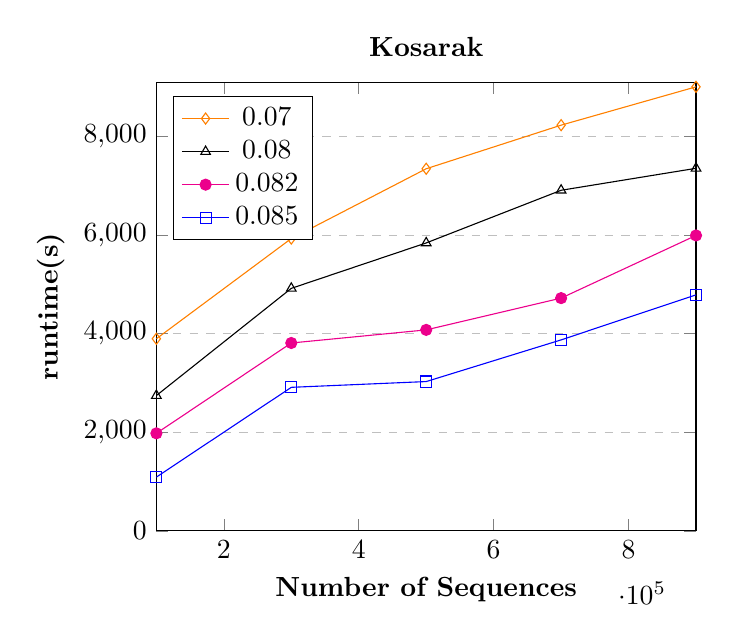
\begin{tikzpicture}
            \begin{axis}[
            title={\textbf{Kosarak}},
            xlabel={\textbf{Number of Sequences}},
            ylabel={\textbf{runtime(s)}},
            xmin=100000, xmax=900000,
            ymin=0, ymax=9100,
            legend pos=north west,
            ymajorgrids=true,
            grid style=dashed,
        ]
            \addplot[
            color=orange,
            mark=diamond,
            ]
            coordinates {
                  (900000,9012)  
                  (700000,8234) 
                  (500000,7349)
                  (300000,5932)
                  (100000,3898)
            };
            \addplot[
            color=black,
            mark=triangle
            ]
            coordinates {
                  (900000,7358)  
                  (700000,6912) 
                  (500000,5843)
                  (300000,4921)
                  (100000,2745)
            };
            \addplot[
            color=magenta,
            mark=*,
            ]
            coordinates {
                  (900000,5995)  
                  (700000,4723) 
                  (500000,4078)
                  (300000,3812)
                  (100000,1978)
            };
            \addplot[
                color=blue,
                mark=square,
                ]
                coordinates {
                  (900000,4789)  
                  (700000,3875) 
                  (500000,3029)
                  (300000,2912)
                  (100000,1090)
                };
            \legend{0.07, 0.08, 0.082, 0.085}   
        \end{axis}
         \end{tikzpicture}
          \end{adjustbox}
          \caption{}
           \end{subfigure}
         \caption{(a)-(g): Runtime Comparison, (h) Scalability Comparisons for IncTree-Miner}
        \label{graph:runtime_scalability_comparison_inc_tree_miner}
\end{figure*}

\textcolor{blue}{Upto now, we have compared with the base proposals related to incremental mining that aligns with the motivation of the proposed solution. Now, we will provide some analysis through comparing with a prominent literature that does not completely aligns with the motivation of the proposed work but goes closely with it, to understand our solution's efficacy in improving runtime.}

\textcolor{blue}{For the comparison MR-INCSPM\cite{saleti2019mapreduce} has been chosen, a Map Reduced framework for ISPM problems. As the proposed solution works for a single machine environment, here for MR-INCSPM such environment has been considered for fair ground analysis. MR-INCSPM worked in backward extension with its own co-occurrence table definition and pruning strategies. So, these factors also provided important points to conduct a critical analysis.} 

\textcolor{blue}{In Fig.\ref{figure:mr_incspm}, we have shown the results for some of the datasets. From the figures, it can be noted that, the performance of IncTree-Miner is comparatively better. The main issue, in single machine based MR-INCSPM is, it generates patterns with sort of prefixspan or database projection alike technique but with backward extension. Here the main improvement factor of ours is faster traversal through links compared to scan based moves. Alongside, their proposed pruning strategies are a subset of the strategies we use for our pruning. So, altogether the performance improvement is achieved.}   

\textcolor{blue}{In \cite{lin2015incrementally}, pre-large concept was proposed where additional set of patterns which are not exactly frequent are pre-computed, so that the number of database re-scans can be reduced. There the authors use additional set of thresholds, upper($s_{u}$) and lower($s_{l}$) minimum support thresholds to perform the additional patterns' pre-computation. The performance of database re-scans can be improved using the proposed IncSP-Tree structure through using its next links and modified next links. These over-computation based approaches suffer greatly when concept drift appears along with the critical selection of the empirically set thresholds.} 

\begin{figure*}[!tb]
        \centering
        \begin{subfigure}{.3\linewidth}
          \centering
           \begin{adjustbox}{max width=\textwidth}
           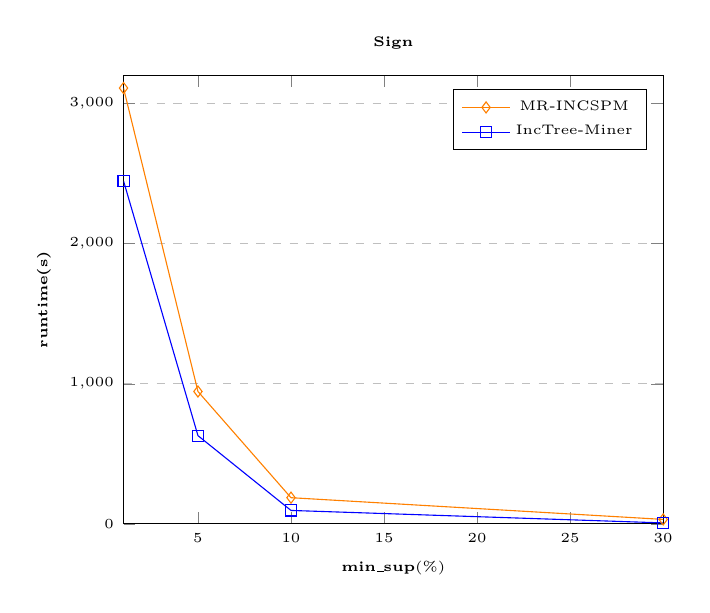
\begin{tikzpicture}
              \begin{axis}[
    title={\textbf{Sign}},
     xlabel={$\textbf{min\_sup}(\%)$},
    ylabel={\textbf{runtime(s)}},
    xmin=1, xmax=30,
    ymin=0, ymax=3200,
    legend pos=north east,
    ymajorgrids=true,
    grid style=dashed,
    legend style={font=\tiny},
    title style={font=\tiny},
    label style={font=\tiny},
    every tick label/.append style={font=\tiny}
]
    \addplot[
    color=orange,
    mark=diamond,
    ]
    coordinates {
            (30, 32) 
            (10, 187)
            (5, 945)
            (1, 3111)
    };
    \addlegendentry{MR-INCSPM}
    
    \addplot[
        color=blue,
        mark=square,
        ]
        coordinates {
            (30, 7) 
            (10, 96)
            (5, 630)
            (1, 2448)
        };
   \addlegendentry{IncTree-Miner}
\end{axis}
           \end{tikzpicture}
          \end{adjustbox}
          \caption{}
         \end{subfigure}
        \begin{subfigure}{.3\linewidth}
          \centering
           \begin{adjustbox}{max width=\textwidth}
           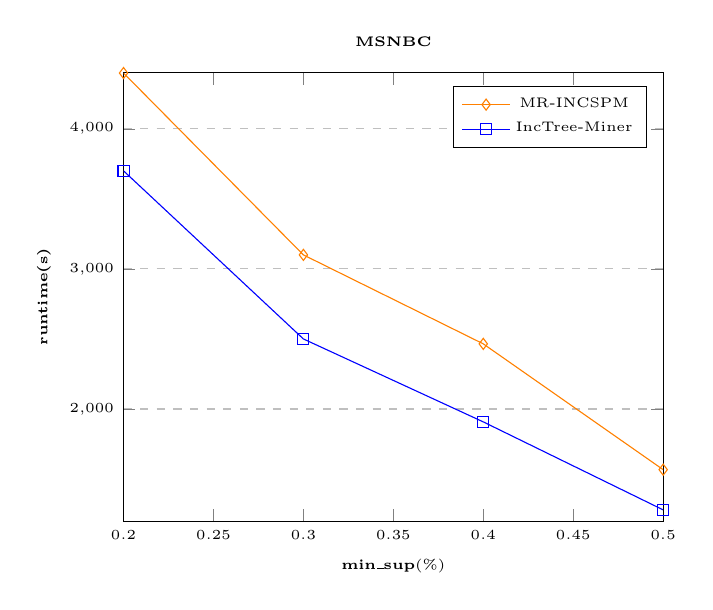
\begin{tikzpicture}
              \begin{axis}[
    title={\textbf{MSNBC}},
    xlabel={$\textbf{min\_sup}(\%)$},
    ylabel={\textbf{runtime(s)}},
    xmin=0.2, xmax=0.5,
    ymin=1200, ymax=4400,
    legend pos=north east,
    ymajorgrids=true,
    grid style=dashed,
    legend style={font=\tiny},
    title style={font=\tiny},
    label style={font=\tiny},
    every tick label/.append style={font=\tiny}
]
    \addplot[
    color=orange,
    mark=diamond,
    ]
    coordinates {
       (0.5, 1567)
       (0.4, 2465)
       (0.3,3100)
       (0.2,4398)
    };
    \addlegendentry{MR-INCSPM}
    
    %tree-miner
    \addplot[
        color=blue,
        mark=square,
        ]
        coordinates {
            (0.5,1280)
            (0.4,1908)
            (0.3,2500)
            (0.2,3700)
        };
   \addlegendentry{IncTree-Miner}
\end{axis}
           \end{tikzpicture}
          \end{adjustbox}
          \caption{}
         \end{subfigure}
        \begin{subfigure}{.3\linewidth}
          \centering
           \begin{adjustbox}{max width=\textwidth}
           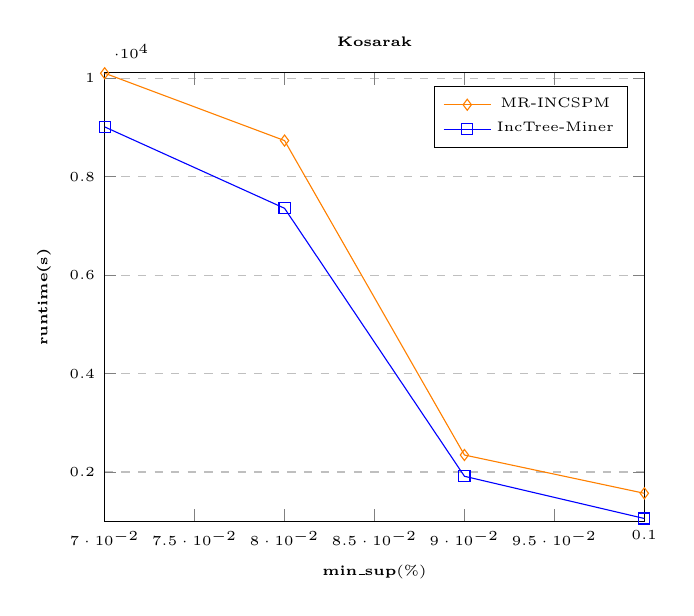
\begin{tikzpicture}
              \begin{axis}[
    title={\textbf{Kosarak}},
     xlabel={$\textbf{min\_sup}(\%)$},
    ylabel={\textbf{runtime(s)}},
    xmin=0.07, xmax=0.1,
    ymin=1000, ymax=10110,
    legend pos=north east,
    ymajorgrids=true,
    grid style=dashed,
    legend style={font=\tiny},
    title style={font=\tiny},
    label style={font=\tiny},
    every tick label/.append style={font=\tiny}
]
    \addplot[
    color=orange,
    mark=diamond,
    ]
    coordinates {
            (0.1, 1567) 
            (0.09, 2345)
            (0.08, 8734)
            (0.07, 10103)
    };
    \addlegendentry{MR-INCSPM}
    
    \addplot[
        color=blue,
        mark=square,
        ]
        coordinates {
            (0.1, 1055) 
            (0.09, 1913)
            (0.08, 7358)
            (0.07, 9012)
        };
    \addlegendentry{IncTree-Miner}  
\end{axis}
           \end{tikzpicture}
          \end{adjustbox}
          \caption{}
         \end{subfigure}
         \caption{Runtime Comparison with MR-INCSPM}
        \label{figure:mr_incspm}
\end{figure*}


\begin{figure*}[!thb]
        \centering
       \begin{subfigure}{.3\textwidth}
          \centering
           \begin{adjustbox}{max width=\textwidth}
           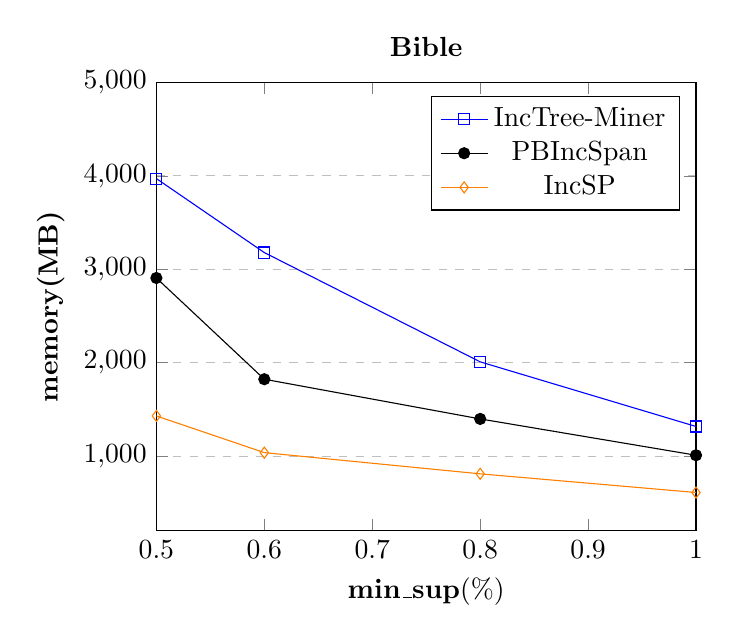
\begin{tikzpicture}
              \begin{axis}[
    title={\textbf{Bible}},
    xlabel={$\textbf{min\_sup}(\%)$},
    ylabel={\textbf{memory(MB)}},
    xmin=0.5, xmax=1,
    ymin=200, ymax=5000,
    legend pos=north east,
    ymajorgrids=true,
    grid style=dashed,
]

% (70, 2456.14 * 2.5 = 6140.25)
% (80, 1331.05 * 2.2 = 2928.31)
% (90, 722.725 * 1.8 = 1300.905)
%prefixspan
    \addplot[
    color=blue,
    mark=square,
    ]
    coordinates {
        (0.5, 3971) 
        (0.6, 3179)
        (0.8, 2009)
        (1, 1317)
    };
    \addlegendentry{IncTree-Miner}  
    %tree-miner
    \addplot[
        color=black,
        mark=*,
        ]
        coordinates {
            (0.5, 2907) 
            (0.6, 1823)
            (0.8, 1398)
            (1,   1009)
        };
    \addlegendentry{PBIncSpan}  
    
    \addplot[
        color=orange,
        mark=diamond,
        ]
        coordinates {
            (0.5, 1430) 
            (0.6, 1037)
            (0.8, 810)
            (1,   610)
        };
    \addlegendentry{IncSP}  
\end{axis}
           \end{tikzpicture}
          \end{adjustbox}
          \caption{}
         \end{subfigure}
        \begin{subfigure}{.3\textwidth}
          \centering
           \begin{adjustbox}{max width=\textwidth}
           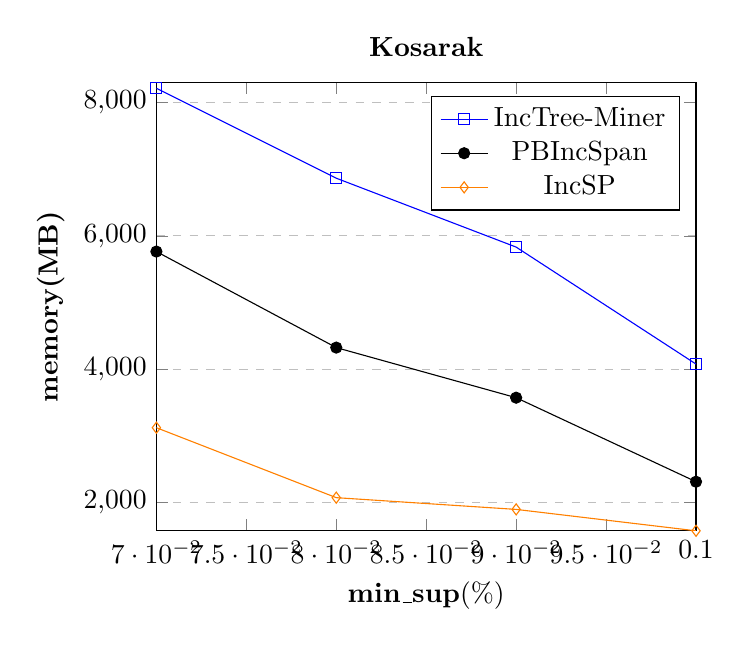
\begin{tikzpicture}
              \begin{axis}[
    title={\textbf{Kosarak}},
    xlabel={$\textbf{min\_sup}(\%)$},
    ylabel={\textbf{memory(MB)}},
    xmin=0.07, xmax=0.1,
    ymin=1578, ymax=8300,
    legend pos=north east,
    ymajorgrids=true,
    grid style=dashed,
]

% (70, 2456.14 * 2.5 = 6140.25)
% (80, 1331.05 * 2.2 = 2928.31)
% (90, 722.725 * 1.8 = 1300.905)
%prefixspan
    \addplot[
    color=blue,
    mark=square,
    ]
    coordinates {
        (0.1, 4078) 
        (0.09, 5832)
        (0.08, 6865)
        (0.07, 8214)
    };
    \addlegendentry{IncTree-Miner}  
    %tree-miner
    \addplot[
        color=black,
        mark=*,
        ]
        coordinates {
            (0.1, 2314) 
            (0.09, 3574)
            (0.08, 4325)
            (0.07, 5765)
        };
    \addlegendentry{PBIncSpan}  
    
    \addplot[
        color=orange,
        mark=diamond,
        ]
        coordinates {
            (0.1, 1578) 
            (0.09, 1899)
            (0.08, 2075)
            (0.07, 3124)
        };
    \addlegendentry{IncSP}  
\end{axis}
           \end{tikzpicture}
          \end{adjustbox}
          \caption{}
         \end{subfigure}
         \begin{subfigure}{.3\textwidth}
          \centering
           \begin{adjustbox}{max width=\textwidth}
           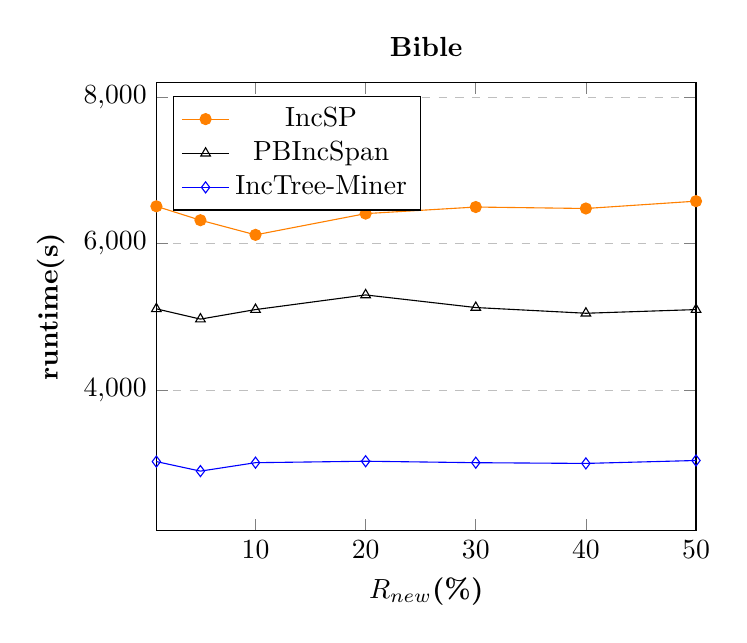
\begin{tikzpicture}
              \begin{axis}[
    title={\textbf{Bible}},
    xlabel={\textbf{$R_{new}$(\%)}},
    ylabel={\textbf{runtime(s)}},
    xmin=1, xmax=50,
    ymin=2080, ymax=8200,
    legend pos=north west,
    ymajorgrids=true,
    grid style=dashed,
]

 \addplot[
    color=orange,
    mark=*,
    ]
    coordinates {
        (1,6510)
        (5,6320)
        (10,6120)
        (20,6410)
        (30,6500)
        (40,6480)
        (50,6580)
    };
    \addlegendentry{IncSP}
    
  \addplot[
    color=black,
    mark=triangle,
    ]
    coordinates {
        (1,5110)
        (5,4970)
        (10,5100)
        (20,5300)
        (30,5128)
        (40,5050)
        (50,5100)
    };
    \addlegendentry{PBIncSpan}
     
   \addplot[
    color=blue,
    mark=diamond
    ]
    coordinates {
         (1,3025)
         (5,2895)
         (10,3010)
         (20,3030)
         (30,3010)
         (40,3000)
         (50,3040)
    };
    \addlegendentry{IncTree-Miner}
\end{axis}
           \end{tikzpicture}
          \end{adjustbox}
          \caption{}
         \end{subfigure}
         \caption{(a)-(b) Memory Evaluation, (c) Performance over $R_{new}$, for IncTree-Miner}
        \label{graph:memory_rnew_comparison_inctree_miner}
\end{figure*}

ISPM algorithms generally need more memory compared to static mining algorithms because they store the frequent patterns' information which is used in the successive iterations. We show a memory usage analysis in Fig. \ref{graph:memory_rnew_comparison_inctree_miner} (a)-(b) over Bible and Kosarak dataset. IncSP stores the support of the prior frequent patterns. So, its memory usage is dependent on the number of frequent patterns. PBIncSpan and IncTree-Miner both keep the previous frequent patterns' support along with their projection information where PBIncSpan uses pseudo projection and IncTree-Miner uses the compact IncSP-Tree node references. But IncTree-Miner stores the sequential database in tree format along with maintaining some data structures leading to comparatively more memory usage than PBIncSpan. As memory usage is directly related to the compactness of the tree, so in dense datasets, this metric's performance is comparatively closer to PBIncSpan. Our incremental solution is the extension of prior proposed static solution and both maintain almost similar types of data structures. In the earlier section, we have discussed how this additional usage gives us significant improvement in mining which also applies here. Being very flexible solution, we have our own memory resilient version. In the memory resilient version, we do not store pattern's projection information which reduces the memory to a great extent with additional time cost during mining.   

Similar to Tree-Miner, we also conducted a scalability test for IncTree-Miner and presented the result over the \textit{Kosarak} dataset in Fig. \ref{graph:runtime_scalability_comparison_inc_tree_miner} (h). We started with few transactions, gradually increased it and recorded the results by varying $min\_sup$. The corresponding figure shows the linear scalability of the solution. To conduct the experiment, we chose $R_{new}=10\%,R_{com}=50\%$ and $R_{prev}=80\%$ over the considered number of transactions. In the Tree-Miner section, we have shown that the structural solution does not create a bottleneck to construct them rather provides improvement in mining time. As IncSP-Tree is an incremental version of SP-Tree it also maintains similar characteristics.   




%Link: https://tex.stackexchange.com/questions/249085/referencing-subfigures-with-subfigure-package

\subsubsection{Effect on Different $R_{new}$ and $R_{com}$}

To evaluate the performance over the ratio of the completely new sequences (new sids) we conducted experiment by varying the percentage of $R_{new}$ over $Bible$ dataset by keeping $R_{com}=50\%$, $R_{prev}=80\%$ and $min\_sup=0.3\%$. We have shown the result in Fig. \ref{graph:memory_rnew_comparison_inctree_miner} (c). We started with $1\%$ and gradually increased it to $30\%$ and we always had two iterations to output the final set of patterns. We wanted to observe if the increased ratio of $R_{new}$ affects the solution's performance or not. From Fig. \ref{graph:memory_rnew_comparison_inctree_miner} (c) it is clear that IncTree-Miner's performance does not degrade due to the $R_{new}$'s increasing ratio compared to PBIncSpan and IncSP. With $R_{new}$'s increment the number of newer patterns' and updated patterns' get increased in the second pass and the number of frequent patterns' get decreased in the first pass. So, in our described scenario, the ISPM algorithm's performance should be almost linear and Fig. \ref{graph:memory_rnew_comparison_inctree_miner} (c) supports our intuition.



Similar to $R_{new}$, we also evaluated our solution by changing the percentage of $R_{com}$. For experiment, we had set $R_{new}=10\%, R_{prev}=80\%$ and varied $R_{com}$ with $min\_sup=0.5\%$. Like the previous discussion, we got almost similar types of results which matched our intuition that IncTree-Miner is not affected due to the increment of the $R_{com}$ and performs comparatively better than PBIncSpan and IncSP.






\subsection{Evaluation of Breadth-First Based Support Counting Technique}

\begin{figure*}[ht]
        \centering
            \begin{adjustbox}{max width=1\textwidth}
             \centering
           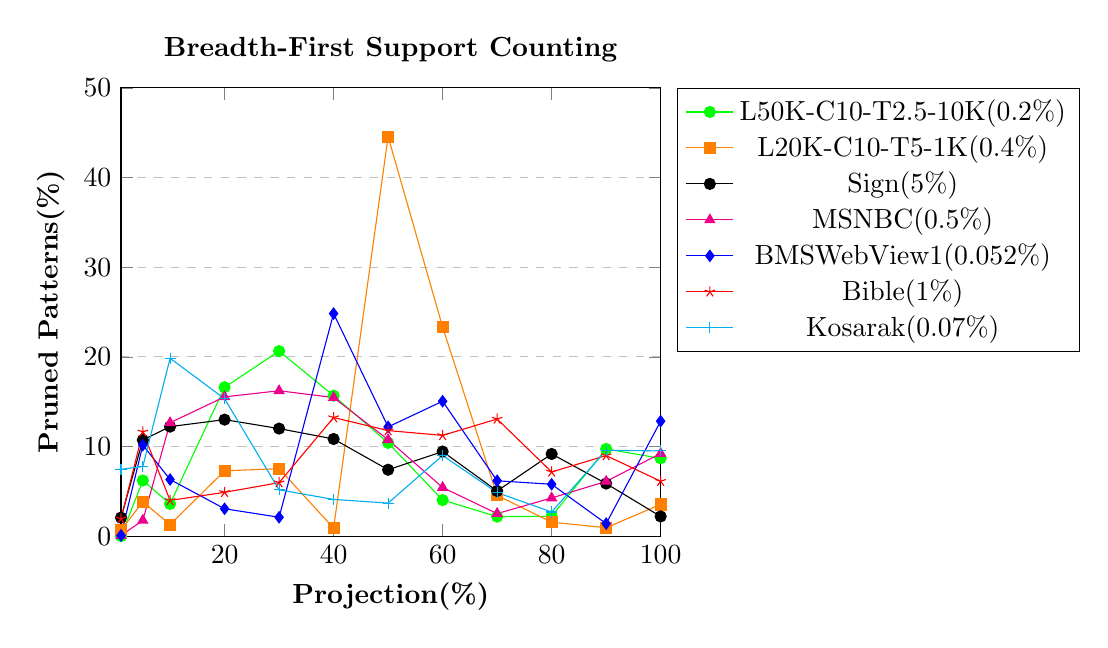
\begin{tikzpicture}
              \begin{axis}[
    title={\textbf{Breadth-First Support Counting}},
    xlabel={\textbf{Projection(\%)}},
    ylabel={\textbf{Pruned Patterns(\%)}},
    xmin=1, xmax=100,
    ymin=0, ymax=50,
    legend pos= outer north east,
    ymajorgrids=true,
    grid style=dashed,
]

\addplot [
    color=green,
    mark=*
    ]
    coordinates {
    (1,0.01)
    (5,6.21)
    (10,3.6)
    (20,16.61)
    (30,20.64) 
    (40,15.67)
    (50,10.41)
    (60,4.03)
    (70,2.18)
    (80,2.22)
    (90,9.73)
    (100,8.68)
    };
    \addlegendentry{L50K-C10-T2.5-10K(0.2\%)}
  
 \addplot [
    color=orange,
    mark=square*
    ]
    coordinates {
    (1,0.67)
    (5,3.84)
    (10,1.29)
    (20,7.29)
    (30,7.53)
    (40,0.9)
    (50,44.56)
    (60,23.32)
    (70,4.55)
    (80,1.56)
    (90,0.95)
    (100,3.54)
    };
    \addlegendentry{L20K-C10-T5-1K(0.4\%)}
    
    \addplot [
    color=black,
    mark=otimes*
    ]
    coordinates {
      (1,2.07)
    (5,10.73)
    (10,12.22) 
    (20,13.0)
    (30,12.0) 
    (40,10.84)
    (50,7.41)
    (60,9.44)
    (70,5.04)
    (80,9.17)
    (90,5.87)
    (100,2.2)
    };
    \addlegendentry{Sign(5\%)}
    
    \addplot [
    color=magenta,
    mark=triangle*
    ]
    coordinates {
        (1,0.07)
        (5,1.77)
        (10,12.65) 
        (20,15.54)
        (30,16.22)
        (40,15.46)
        (50,10.76)
        (60,5.43)
        (70,2.52)
        (80,4.26)
        (90,6.11)
        (100,9.22)
    };
    \addlegendentry{MSNBC(0.5\%)}
    
    \addplot [
    color=blue,
    mark=diamond*
    ]
    coordinates {
        (1,0.09)
        (5,10.16)
        (10,6.32)
        (20,3.06)
        (30,2.11)
        (40,24.83)
        (50,12.19)
        (60,15.05)
        (70,6.18)
        (80,5.79)
        (90,1.4)
        (100,12.83)
    };
    \addlegendentry{BMSWebView1(0.052\%)}
    
    \addplot [
        color=red,
        mark=star
        ]
        coordinates {
         (1,1.93)
        (5,11.64)
        (10,3.99)
        (20,4.89)
        (30,5.97)
        (40,13.23)
        (50,11.78) 
        (60,11.24)
        (70,13.07)
        (80,7.16)
        (90,8.99)
        (100,6.13)
        };
        \addlegendentry{Bible(1\%)}
        \addplot [
        color=cyan,
        mark=+
        ]
        coordinates {
        (1,7.46)
        (5,7.77)
        (10,19.84)
        (20,15.33)
        (30,5.17)
        (40,4.1)
        (50,3.69)
        (60,9.0)
        (70,4.86)
        (80,2.7)
        (90,9.58)
        (100,9.51)
        };
        \addlegendentry{Kosarak(0.07\%)}
\end{axis}
           \end{tikzpicture}
           \end{adjustbox}
         \caption{Evaluation of Breadth-First Based Support Counting Technique}
        \label{graph:breadth-first-support}
\end{figure*}

In this section, we will evaluate the performance of the proposed breadth-first based support counting technique to understand how fast it can detect an infrequent pattern and stop support counting. To guide our mining process we use the co-occurrence information of the items stored in $sList$ and $iList$. With the suffix extension of the pattern these two lists shrink. During support calculation of the extensions, we discover some patterns' infrequency. The algorithm's runtime improves depending on how quickly it is able to detect the infrequency rather than performing complete projection. In Fig. \ref{graph:breadth-first-support}, we present an analysis to understand how quickly our proposed pruning technique detects infrequent patterns. In the x-axis, we have provided the percentage value of the projection size and in the y-axis, we have provided the percentage of infrequent patterns been detected. For example, in the \textit{L20-C10-T2.5-10K} dataset, at 50\% value in the x-axis, we get a 45\% value in the corresponding y-axis, which denotes that, of all the infrequent patterns been tested, 45\% of them are detected performing only 50\% projection of their corresponding complete projected database. From, Fig. \ref{graph:breadth-first-support}, it is clear that our proposed support counting technique is able to detect most of the infrequent patterns without performing a complete projection of the underlying sub-database. We have shown the corresponding $min\_sup$ values beside each legend in Fig. \ref{graph:breadth-first-support}.  The figure is generated by executing Tree-Miner.



\subsection{Effectiveness in Interactive Mining}
The proposed SP-Tree structures hold ``build-once-mine-many" property which states that the structures are capable of performing multiple mining iterations based on users' requests without bringing any change to the existing structures for different $min\_sup$ values.

The most difficult scenario in interactive mining is, the gradual decrease in $min\_sup$  ($20\% \,\to\, 10\% \,\to\, 5\%$, etc) where with this decrease a new set of previously infrequent patterns may become frequent. So, to discover those patterns, we need to perform a mining iteration. Here, using BPFSP-Tree's patterns' projection information we can efficiently discover the newly frequent patterns which will be the super patterns (apriori property) of existing frequent patterns. Through projection information, we can directly reach a pattern's corresponding nodes and start expanding from there using the next links. In Table \ref{table:interactive_mining_descending_minsup}(second group of column) we have shown some results related to this scenario. If, we had to start mining from scratch then the time usage would have increased significantly. Here the mining time gets reduced because already a group of patterns have been calculated alongside can use projection information and faster pattern search procedure. 

\begin{table*}[!htbp]
\centering
%% increase table row spacing, adjust to taste
%\renewcommand{\arraystretch}{1.3}
% if using array.sty, it might be a good idea to tweak the value of
% \extrarowheight as needed to properly center the text within the cells
%\centering
%% Some packages, such as MDW tools, offer better commands for making tables
%% than the plain LaTeX2e tabular which is used here.
\begin{tabular}{|l|l|l|l|l|l|l|l|l|l|}
\hline
 Dataset & \multicolumn{5}{l|}{Descending $min\_sup$}  & \multicolumn{4}{l|}{Ascending $min\_sup$} \\ 
 \hline
 Bible & $min\_sup(\%)$ & 10 & 1 & 0.8 & 0.5 & 0.5 & 0.8 & 1 & 5\\
 & T(sec.) & 228.2 & 579.2 & 675 & 935.5 &  2907 & 0.0008 & 0.0007 & 0.0003\\
 \hline
 BMSWebView1 & $min\_sup(\%)$ & 0.06 & 0.055 & 0.052 & 0.05 & 0.05 & 0.052 & 0.055 & 0.06 \\  
 & T(sec.) & 19.8 & 71 & 226.5 & 865.2 & 1321 & 5.7 & 1.1 & 0.7  \\
 \hline
 Sign & $min\_sup(\%)$ & 30 & 10 & 5 & 1 & 1  & 5 & 10 & 30 \\  
 & T(sec.) & 19.8 & 71 & 226.5 & 865.2 & 1 & 5 & 10 & 30 \\ 
 \hline
 MSNBC & $min\_sup(\%)$ &  0.085 & 0.08 & 0.075 & 0.07 & 0.2 & 0.3 & 0.35 & 0.4 \\
 & T(sec.) & 1037.4 & 492.7 & 829 & 742.2 & 3700 & 0.4 & 0.3 & 0.2 \\ 
 \hline
 Kosarak & $min\_sup(\%)$ &0.085 & 0.08 & 0.075 & 0.07 & 0.07 & 0.075 & 0.08 & 0.085\\
 & T(sec.) & 3037.3 & 2512 & 1231.4 & 1021.3 & 7925 & 5.1 & 3.05 &0.98 \\
 \hline
 L20-C10-T5-N1K & $min\_sup(\%)$ & 0.04 & 0.035 & 0.03 & 0.025  & 0.025 & 0.03 & 0.035 & 0.04 \\
 & T(sec.) & 313.7 & 221.5 & 325.3 & 710 & 1012 & 1.14 & 0.08 & 0.07 \\
 \hline
 L50-C10-T2.5-N10K & $min\_sup(\%)$ & 0.031 & 0.03 & 0.025 & 0.02 & 0.02 & 0.025 & 0.03 & 0.031 \\
 & T(sec.) & 313.7 & 221.5 & 325.3 & 710 & 2010 & 0.2 & 0.11 & 0.05 \\
 \hline
\end{tabular}
\caption{Interactive Mining: Performance in Descending $min\_sup$ and Ascending $min\_sup$.}
\label{table:interactive_mining_descending_minsup}
\end{table*}

The best case scenario, in interactive mining comes from the gradual increase in $min\_sup$ ($5\% \,\to\, 10\% \,\to\, 20\% $, etc) where with this increase no new patterns become frequent rather a group of previously frequent patterns may become infrequent. To efficiently remove these newly infrequent patterns, we can use Bottom-up traversal strategy of BPFSP-Tree which will help traverse lesser patterns in this regard. In Table \ref{table:interactive_mining_descending_minsup}(third group of column), we have shown some results related to this scenario.  



%An example can be used to understand the concept. Suppose, in a database, we have a pattern $(a)(b)$ lying in 100 transactions. We have minimum support threshold value as 90 and we want to check extension for $c(ex - (a)(b)(c))$ in $(a)(b)$'s projected database where $(a)(b)(c)$'s actual support value is 70. In our breadth-first solution, we remove a node and add its subtree during pattern extension, gradually reducing the support count. So, our approach might check only 10\% or 10 transactions($\sim10\%$) or 10\% of the total underlying subtrees and understand that $(a)(b)(c)$'s support will fall under 95 and thus will stop from further projecting. 


\subsection{Analytical Novelty of IncTree-Miner with IncSP-Tree}
Our proposed SP-Tree and IncSP-Tree provides an efficient structural manner to store the the sequential database leading to an overall improved runtime during mining. Our proposed Tree-Miner is an efficient algorithm to mine sequential patterns from static database and our proposed IncTree-Miner is an efficient algorithm to solve the incremental mining problem. IncTree-Miner's performance depends on single support threshold parameter where as some literature have adopted buffering concepts \cite{cheng2004incspan}, multiple threshold based concepts \cite{lin2015incrementally} to solve the ISPM problem. Main problems of these approaches are, their performance solely depends on these empirically set thresholds' values. As it is difficult to guess the database characteristics prior, it is very difficult to set these additional parameters appropriately which leads to additional complexity and wastage in both memory and runtime as they might need to pre-compute and store huge amount of infrequent (or can be regarded as semi-frequent) patterns' information which might never get frequent. Also, these approaches are severely affected due to seasonal concept drift. Concept drift basically indicates the sudden shifting in frequent patterns' distribution where a huge number of previously infrequent patterns suddenly become frequent and most of the previously over-computed semi-frequent patterns also do not bear that transition characteristics. In this case, the existing additional parameter based solutions have to re-mine the complete raw database to discover such patterns.   

But as our designed solutions store the databases in a structured format, here pattern searching is comparatively faster. Also by storing the projection information of the frequent patterns, we get an advantage to efficiently track the newer frequent patterns which are super patterns of the existing ones. As, we did not perform the over computations to calculate the information of the semi-frequent patterns which could not help much here, that cost also does not add in our solution. Moreover, our proposed structure stores the complete database in a compact format. So, it is able to handle the absence of prior database in stream mining and runtime threshold parameter change. Also, our solution is able to mine patterns based on user's requests at anytime having no dependency of mining after each iteration. Our proposed tree-based technique is a new approach to solve sequential mining problem. So, our solution can also be fitted to other extra parameter based approaches, e.g., when those approaches would need to re-mine the database, they can use our proposed SP-Tree structures to faster traverse in the database along with generating the patterns.  



